










% PLEASE DO NOT PLAY WITH ALL THESE SETTINGS, UNLESS YOU REALLY KNOW WHAT YOU ARE DOING. 

%IF YOU HAVE ANY QUESTIONS PLEASE CONTACT: Oscar Vega <ovega@csufresno.edu>

%LaTeX file, comments, and Fresno State formatting created and developed by Brent Alexander Wilson: snahhan@gmail.com.
%Thanks to Dr. Gerardo Munoz for initially creating the formatting of the title, approval, and authorization for reproduction pages.
%Last Updated: November 2012 (GM).
%Last Modified: Oscar Vega, August 2021.
\documentclass[12pt,leqno]{article}\usepackage[pdftex]{graphicx}\usepackage[usenames,dvipsnames]{xcolor}
% maxwidth is the original width if it is less than linewidth
% otherwise use linewidth (to make sure the graphics do not exceed the margin)
\makeatletter
\def\maxwidth{ %
  \ifdim\Gin@nat@width>\linewidth
    \linewidth
  \else
    \Gin@nat@width
  \fi
}
\makeatother

\definecolor{fgcolor}{rgb}{0.345, 0.345, 0.345}
\newcommand{\hlnum}[1]{\textcolor[rgb]{0.686,0.059,0.569}{#1}}%
\newcommand{\hlsng}[1]{\textcolor[rgb]{0.192,0.494,0.8}{#1}}%
\newcommand{\hlcom}[1]{\textcolor[rgb]{0.678,0.584,0.686}{\textit{#1}}}%
\newcommand{\hlopt}[1]{\textcolor[rgb]{0,0,0}{#1}}%
\newcommand{\hldef}[1]{\textcolor[rgb]{0.345,0.345,0.345}{#1}}%
\newcommand{\hlkwa}[1]{\textcolor[rgb]{0.161,0.373,0.58}{\textbf{#1}}}%
\newcommand{\hlkwb}[1]{\textcolor[rgb]{0.69,0.353,0.396}{#1}}%
\newcommand{\hlkwc}[1]{\textcolor[rgb]{0.333,0.667,0.333}{#1}}%
\newcommand{\hlkwd}[1]{\textcolor[rgb]{0.737,0.353,0.396}{\textbf{#1}}}%
\let\hlipl\hlkwb

\usepackage{framed}
\makeatletter
\newenvironment{kframe}{%
 \def\at@end@of@kframe{}%
 \ifinner\ifhmode%
  \def\at@end@of@kframe{\end{minipage}}%
  \begin{minipage}{\columnwidth}%
 \fi\fi%
 \def\FrameCommand##1{\hskip\@totalleftmargin \hskip-\fboxsep
 \colorbox{shadecolor}{##1}\hskip-\fboxsep
     % There is no \\@totalrightmargin, so:
     \hskip-\linewidth \hskip-\@totalleftmargin \hskip\columnwidth}%
 \MakeFramed {\advance\hsize-\width
   \@totalleftmargin\z@ \linewidth\hsize
   \@setminipage}}%
 {\par\unskip\endMakeFramed%
 \at@end@of@kframe}
\makeatother

\definecolor{shadecolor}{rgb}{.97, .97, .97}
\definecolor{messagecolor}{rgb}{0, 0, 0}
\definecolor{warningcolor}{rgb}{1, 0, 1}
\definecolor{errorcolor}{rgb}{1, 0, 0}
\newenvironment{knitrout}{}{} % an empty environment to be redefined in TeX

\usepackage{alltt}
\usepackage{amsmath,amssymb,comment,amsthm}
\usepackage{latexsym}
\usepackage{nextpage}
%\usepackage[pdftex]{graphicx}   %just in case graphicx is not enough... shouldn't need this
\usepackage{graphicx}
\usepackage{thmtools}
\usepackage{float}
\usepackage{array,multirow,hhline}%for tricky things with tables

%%%%%%%%%%%%%%%%%%%%%%%%%%%%%%%%%%%%%%%%%%%%%%%%%%%%%%%%%%%%%%%%%%
%%%%%%%%%%%%%%%%%%%%%%%%%%%%%%%%%%%%%%%%%%%%%%%%%%%%%%%%%%%%%%%%%%
%%%%%%%%%%%                                        Fresno State Formatting Requirements Begins                                  %%%%%%%%%%%%
%%%%%%%%%%%%%%%%%%%y%%%%%%%%%%%%%%%%%%%%%%%%%%%%%%%%%%%%%%%%%%%%%%%
%%%%%%%%%%%%%%%%%%%%%%%%%%%%%%%%%%%%%%%%%%%%%%%%%%%%%%%%%%%%%%%%%%

\usepackage{tocloft} %For table of contents.
\usepackage{verbatim} %Allows us to use \setcounter for manipulating pages
\usepackage{setspace} %Lets user change line spacing of text: normal, 1.5x, and double
\usepackage{indentfirst} %Allow first paragraph to be indented in sections/subsections
\usepackage[font=normal,labelfont=normal,labelsep=period,tableposition=top,justification=raggedright]{caption} %Do a little magic to captions
\usepackage{flafter} %Ensure floats (tables/figures) are never placed before their references.
\usepackage{mathrsfs} %For math symbols -- script L for luminosity
\usepackage{ragged2e} %Used to enable command \raggedright
%\usepackage[compact]{titlesec} %Used for titlespacing command.

\clubpenalty10000
\widowpenalty10000
%those are for avoiding orphan lines at top of pages

\raggedright%Enables left adjust of all text and gets rid of hyphenation throughout the paper, which is required for Fresno formatting.

%This disables bold text on section titles and sets the spacing before & after of section title


\makeatletter
\renewcommand\section{\@startsection {section}{1}{\z@}%
{-3.5ex \@plus -1ex \@minus -.2ex}%
{2.3ex \@plus.2ex}%
{\normalfont\centering}}
\makeatother




%This disables bold text on subsection titles and sets the spacing before & after of section title
\makeatletter
\renewcommand\subsection{\@startsection {subsection}{1}{\z@}%
{-3.5ex \@plus -1ex \@minus -.2ex}%
{0.8pt plus 2pt minus 2pt}%
{\normalfont}}
\makeatother

%This disables bold text on subsubsection titles and sets the spacing before & after of section title
\makeatletter
\renewcommand\subsubsection{\@startsection {subsubsection}{1}{\z@}%
{-3.5ex \@plus -1ex \@minus -.2ex}%
{0.8pt plus 2pt minus 2pt}%
{\normalfont}}
\makeatother

\newcommand{\usubsection}[1]{\subsection[#1]{\centering\normalfont\underline{#1}}}% This underlines sub-sections -- must use \usubsection in paper to identify!
\newcommand{\usubsubsection}[1]{\subsubsection[#1]{\normalfont\normalfont\underline{#1}}}% This underlines sub-sub-sections -- must use \usubsubsection in paper to identify!

\setcounter{tocdepth}{2}%Don't show subsubsections in the Table of Contents:
\setcounter{secnumdepth}{-1}%Disables chapter, section, and subsection numbering
\setlength{\parindent}{0.5in}%Paragraphs must be indented 1/2"
\setlength{\cftbeforefigskip}{0.3cm}% Space between elements of the List of Figures
\setlength{\cftbeforetabskip}{0.3cm}% Space between elements of the List of Tables
\setlength{\cftbeforesecskip}{0.3cm}% Space before Section entries in the Table of Contents
\setlength{\cftbeforesubsecskip}{0.3cm}% Space before Sub-Section entries in the Table of Contents
\setlength\headsep{12pt}%Change spacing between page number and top of text
\setlength{\cftfignumwidth}{1.5em}%Change space between Figure X and the caption for it on the List of Figures
\setlength{\cfttabnumwidth}{1.5em}%Change space between Table X and the caption for it on the List of Tables

\renewcommand{\contentsname}{TABLE OF CONTENTS} %Renames table of contents to how you want it:
\renewcommand{\cfttoctitlefont}{\centering\normalfont}%Change Table of Contents title to be normal & not bold
\renewcommand{\cftsecleader}{\cftdotfill{\cftdotsep}}%This gives you the dots for the table of contents page:
\renewcommand{\listtablename}{LIST OF TABLES}%Renames table of tables to how you want it:
\renewcommand{\cftlottitlefont}{\centering\normalfont}%Change List of Tables title to be normal & not bold
\renewcommand{\cfttabfont}{Table }%Renames "1" on list of tables to "Table 1":
\renewcommand{\listfigurename}{LIST OF FIGURES}%Renames table of figures to how you want it:
\renewcommand{\cftloftitlefont}{\centering\normalfont}%Change List of Figures title to be normal & not bold
\renewcommand{\cftfigfont}{Figure }%Renames "1" on list of figures to "Figure 1":
\renewcommand{\refname}{REFERENCES}%Renames references to how you want it:
\renewcommand{\cftfigaftersnum}{.}%Add a period after Figure X in List of Figures
\renewcommand{\cfttabaftersnum}{.}%Add a period after Table X in List of Tables

%Use this to put page numbers at top right of page
\usepackage{fancyhdr}
\fancyhf{}
\renewcommand{\headrulewidth}{0pt} % remove the header rule
\rhead{\thepage}
\pagestyle{fancy}
\fancyheadoffset[HR]{0.02in}%Moves (horizontally) the page number                              
%KEEP ALL THIS TOGETHER

% Change Table of Content section headers and page numbers to normal instead of bold font
\renewcommand{\cftsecfont}{\normalfont}
\renewcommand{\cftsecpagefont}{\normalfont}

%%Change margins \marginsize{left}{right}{top}{bottom}:
\usepackage{anysize}
\marginsize{1.7in}{1in}{1.2in}{1.6in}

%%%%%%%%%%%%%%%%%%%%%%%%%%%%%%%%%%%%%%%%%%%%%%%%%%%%%%%%%%%%%%%%%%
%%%%%%%%%%%%%%%%%%%%%%%%%%%%%%%%%%%%%%%%%%%%%%%%%%%%%%%%%%%%%%%%%%
%%%%%%%%%%%%                                   Fresno State Formatting Requirements Ends                                   %%%%%%%%%%%%%
%%%%%%%%%%%%%%%%%%%%%%%%%%%%%%%%%%%%%%%%%%%%%%%%%%%%%%%%%%%%%%%%%%
%%%%%%%%%%%%%%%%%%%%%%%%%%%%%%%%%%%%%%%%%%%%%%%%%%%%%%%%%%%%%%%%%%

%%%%%%%%%%%%%%%%%%%%%%%%%%%%%%%%%%%%%%%%%%%%%%%%%%%%%%%%%%%%%%%%
%BEGIN OF MATH SYMBOLS AND COMMANDS
% You, most probably, don't need all what follows. Comment out whatever you don't need to better run LaTeX.
\usepackage[all]{nowidow} %this is to avoid orphan lines
\usepackage{array}
\usepackage[usenames,dvipsnames]{xcolor}
\usepackage{tikz}
%\usepackage{subfigure}

\newtheorem{lemma}{Lemma}%[chapter]
\newtheorem{theorem}[lemma]{Theorem}
\newtheorem{corollary}[lemma]{Corollary}
\newtheorem{proposition}[lemma]{Proposition}
\newtheorem{defnition}[lemma]{Definition} %leave this as is, soon this will be redefined as a new environment
\newtheorem{example}[lemma]{Example}
\newenvironment{definition}{\begin{defnition} \em}{\end{defnition}}

\theoremstyle{remark}
\newtheorem{remark}[theorem]{Remark}

\newcommand{\close}[1]{\begin{equation} #1 \tag*{$\Box$} \end{equation}}

\newcommand{\wtilde}{\widetilde}
\newcommand{\what}{\widehat}
\newcommand{\n}{\noindent}
\renewcommand{\bar}{\overline}
%\newcommand{\qed}{\hfill $\square$}%%%%%%%%%%%%%%%%%%%%%%% use \qed to get square at the end of proofs.
%\newcommand{\proof}{\n \emph{\underline{Proof}} \ : \ }
\newcommand{\rbox}{\hfill $\Box$}
\newcommand{\rdef}{\mbox{} \hfill $\rhd$}
\newcommand{\la}{\langle}
\newcommand{\ra}{\rangle}
\newcommand{\normal}{\unlhd}
\newcommand{\subnormal}{\unlhd \unlhd}
\newcommand{\kar}{\stackrel{\mathrm{char}}{\normal}}
\newcommand{\lra}{\Leftrightarrow}
\newcommand{\labelpar}[1]{\label{#1}}
\newcommand{\Image}{\mbox{\rm Im} \,}
\newcommand{\Ker}{\mbox{\rm Ker} \,}
\renewcommand{\Im}{\mbox{\rm Im} \,}
\newcommand{\deq}{\stackrel{\mathrm{def}}{=}}
\newcommand{\ds}{\displaystyle}
\newcommand{\tst}{\textstyle}
\newcommand{\mbf}{\mathbf}
\newcommand{\mbb}[1]{\mbox{\boldmath$#1$}}
\newcommand{\con}{\, | \,}
\newcommand{\mb}[1]{{\mathbb #1}}
\newcommand{\ip}[2]{\left\langle #1, #2 \right\rangle}
\newcommand{\solution}{\emph{Solution : }}
\newcommand{\answer}[1]{\begin{center} \framebox{#1} \end{center}}
\newcommand{\eps}{\varepsilon}
\newcommand{\boxform}[1]{\medskip \mbox{} \hfill #1 \hfill $\Box$}
\newcommand{\der}[2]{\ds{\frac{\partial #1}{\partial#2}}}
\newcommand{\se}[1]{\setlength{\extrarowheight}{#1}}
\newcommand{\Der}[2]{\frac{\partial #1}{\partial#2}}
\newcommand{\Aut}{\mbox{\rm Aut}}
\newcommand{\Out}{\mbox{\rm Out}}
\newcommand{\Inn}{\mbox{\rm Inn}}
\newcommand{\Sym}{\mbox{\rm Sym}}
\newcommand{\Alt}{\mbox{\rm Alt}}
\newcommand{\GL}{\mbox{\rm GL}}
\newcommand{\PGL}{\mbox{\rm PGL}}
\newcommand{\SL}{\mbox{\rm SL}}
\newcommand{\PSL}{\mbox{\rm PSL}}
\newcommand{\SU}{\mbox{\rm SU}}
\newcommand{\PSU}{\mbox{\rm PSU}}
\newcommand{\symp}{\mbox{\rm Sp}}
\newcommand{\psymp}{\mbox{\rm PSp}}
\newcommand{\unit}{\mbox{\rm U}}
\newcommand{\orth}{\mbox{\rm O}}
\newcommand{\proj}{\mbox{\rm P}}
\newcommand{\Syl}{\mbox{\rm Syl}}
\newcommand{\End}{\mbox{\rm End}}
\newcommand{\rank}{\mbox{\rm rank}}
\newcommand{\Sol}{\mbox{\rm Sol}}
\newcommand{\Fit}{\mbox{\rm Fit}}
\newcommand{\Frat}{\mbox{\rm Frat}}
\newcommand{\Matr}{\mbox{\rm Matr}}
\newcommand{\rad}{\mbox{\rm rad}}
\newcommand{\ord}{\mbox{\rm ord}}
\newcommand{\Fix}{\mbox{\rm Fix}}
\newcommand{\N}{\mathbb{N}}
\newcommand{\F}{\mathbb{F}}
%\newcommand{\emptypage}{\newpage \thispagestyle{empty} \begin{tabbing} just an empty page  \kill \end{tabbing}}
\renewcommand{\liminf}{ \underline{\lim} \,}
\renewcommand{\limsup}{\overline{\lim} \,}
\renewcommand{\iff}{\Leftrightarrow}
\renewcommand{\Re}[1]{\mbox{\rm Re}(#1)}
\renewcommand{\Im}[1]{\mbox{rm Im}(#1)}
\newcommand{\Log}{\mbox{\rm Log} \, }
\newcommand{\hs}{\hspace{1mm}}
\newcommand{\tcr}{\textcolor{red}}
%\renewcommand{\thetable}{\Roman{table}}  To make tables numbered using roman numerals
\newcommand*\mycirc[1]{
\begin{tikzpicture}[baseline=(C.base)]
\node[draw,circle,inner sep=1pt](C) {#1};
\end{tikzpicture}}
%%%%%%%%%%%%%%%%%%%%%%%%%%%%%%%%%%%%%%%%%%%%%%%%%%%%%%%%%%%%%%%%
%END OF MATH SYMBOLS AND COMMANDS

%%%%%%%%%%%%%%%%%%%%%%%%%%%%%%%%%%%%%%%%%%%%%%%%%%%%%%%%%%%%%%%%

\IfFileExists{upquote.sty}{\usepackage{upquote}}{}
\begin{document}
%%%%%%%%%%%%%%%%%%%%%%%%%%%%%%%%%%%%%%%%%%%%%%%%%%%%%%%%%%%%%%%%
\begin{center}
ABSTRACT
\end{center}

\begin{center}
%ABSTRACT TITLE
%SAME TITLE AS TITLE PAGE, SINGLE-SPACED IF OVER \newline
%ONE LINE, TYPED IN INVERTED PYRAMID FORM
Predicting NCAA March Madness Outcomes
\end{center}

\doublespacing
The aim of this project is to develop a machine learning framework to predict outcomes for the NCAA Division I Mens Basketball Tournament. The purpose is to build upon traditional statistical rankings by implementing an automated pipeline that generates precise win probabilities for every possible tournament matchup. Extensive research into historical sports forecasting and modern machine learning techniques was conducted to establish a baseline for predictive accuracy and model calibration.

Following a comprehensive review of existing literature, the models were constructed using R. The primary dataset includes historical game results and Massey Ordinals, supplemented by custom feature engineering designed to capture team momentum and efficiency metrics. Four different modeling techniques were evaluated on the training data: Logistic Regression, Linear Regression, Random Forest, and XGBoost.
 
Unlike standard classification tasks, the final model was evaluated based on its ability to minimize the Brier Score, ensuring that the predicted probabilities were well calibrated against actual tournament results. The findings indicate that the integration of ensemble methods and strength of schedule adjustments provides a competitive edge in forecasting the high variance environment of the tournament. The complete codebase and dataset configurations are hosted on GitHub for further research and reproducibility. (do i put the link here or somewhere else)

%The abstract should fit on one page. A blank guard sheet should follow. Neither of these pages receives a page number, and neither is considered part of the project proper. 

\singlespacing
\vskip 0.3in
\noindent Jonathen Marin%ABSTRACT AUTHOR NAME

\noindent May 2026 %Use May or December, depending on the semester you graduate, even though the deadline is earlier than that.
\thispagestyle{empty}
\newpage

%%%%%%%%%%%%%%%%%%%%%%%%%%%%%%%%%%%%%%%%%%%%%%%%%%%%%%%%%%%%%%%%
%BLANK PAGE AFTER ABSTRACT
\mbox{}
\thispagestyle{empty}
\newpage

%%%%%%%%%%%%%%%%%%%%%%%%%%%%%%%%%%%%%%%%%%%%%%%%%%%%%%%%%%%%%%%%
\begin{center}
%PROJECT TITLE THAT EXTENDS OVER ONE LINE TYPED IN INVERTED PYRAMID FORM. JUST LIKE IN ABSTRACT
Predicting NCAA March Madness Outcomes
\end{center}

\vskip 2in

\begin{center}
by
\end{center}

\begin{center}
Jonathen Marin%AUTHOR'S FULL NAME
\end{center}

\vskip 2in

\begin{center}
A project \\[6pt]
submitted in partial \\[6pt]
fulfillment of the requirements for the degree of \\[6pt]
Master of Science in Mathematics \\[6pt]
in the College of Science and Mathematics \\[6pt]
California State University, Fresno
\end{center}

\begin{center}
May 2026 %CHECK DATE
\end{center}
\setcounter{page}{1}
\pagenumbering{roman}
\thispagestyle{empty}
\newpage

%%%%%%%%%%%%%%%%%%%%%%%%%%%%%%%%%%%%%%%%%%%%%%%%%%%%%%%%%%%%%%%%
\begin{center}
APPROVED
\end{center}

\begin{center}
For the Department of Mathematics:
\end{center}

%Note: Do not use academic titles (i.e., Dr., Ph.D.) when you enter your committee members' names on this page.  Use first and last name only.  When filling in the department name, do not use "Department of"  Simply use Mathematics.  Laser-print this page.  Inkjet print is not acceptable.  Once your committee members have signed, you can bring it to the Graduate Office (Madden Library 4th floor) and I will secure the dean's signature for you.  Delete this box after you have read the instructions.

\noindent
%We use the quote to move the block of text over so it looks nice and aligned with lines below
\begin{quote}
We, the undersigned, certify that the project of the following student meets the required standards of scholarship, format, and style of the university and the student's graduate degree program for the awarding of the master's degree.
\end{quote}

\vskip 0.5in

\begin{center}
Jonathen Marin  %TYPE STUDENT'S NAME THERE. TYPED SAME AS ON TITLE PAGE
\vskip -0.1in
\makebox[\textwidth]{\hspace{4pc}\hrulefill\hspace{4pc}}
Project Author
\end{center}

\vskip 0.5in

\begin{center}
 \makebox[\textwidth]{\hspace{2pc}\hrulefill\hspace{2pc}}
 \end{center}
 \vskip -0.2in
 \hspace{2pc}%TYPE CHAIRPERSON'S  NAME THERE
Earvin Balderama (Chair) \hfill Mathematics  \hspace{2pc}

%THE REST SHOW UP IN ALPHABETICAL ORDER

\vskip 0.3in
\begin{center}
 \makebox[\textwidth]{\hspace{2pc}\hrulefill\hspace{2pc}}
 \end{center}
 \vskip -0.2in
 \hspace{2pc}%TYPE COMMITTEE MEMBER NAME THERE
Patrick Chung \hfill Mathematics  \hspace{2pc}

\vskip 0.3in
\begin{center}
\makebox[\textwidth]{\hspace{2pc}\hrulefill\hspace{2pc}}
\end{center}
\vskip -0.2in
\hspace{2pc}%TYPE COMMITTEE MEMBER NAME THERE
Mario Bañuelos \hfill Mathematics \hspace{2pc}   %TYPE DEPARTMENT NAME OR PROFESSIONAL AFFILIATION, IN CASE COMMITTEE MEMBER IS NOT IN THE DEPARTMENT OF MATHEMATICS

\thispagestyle{empty}
\newpage

%%%%%%%%%%%%%%%%%%%%%%%%%%%%%%%%%%%%%%%%%%%%%%%%%%%%%%%%%%%%%%%%
\begin{center}
ACKNOWLEDGMENTS
\end{center}
\doublespacing

I would like to thank my advisor, Dr. Dvisor, for her helpful advice, guidance, knowledge, and overall general brilliance. It was an honor for me to have the chance to work with such a great mind. I would also like to thank all project committee members for, hopefully, having read my work and asking easy questions at my defense. I  also thank my parents....
\newline\newline\newline

\singlespacing
\thispagestyle{empty}
\newpage

%%%%%%%%%%%%%%%%%%%%%%%%%%%%%%%%%%%%%%%%%%%%%%%%%%%%%%%%%%%%%%%%
\addtocontents{toc}{\hfill Page\par}%This adds text "Page" to Table of Contents

%This creates the table of contents page automatically
\begin{center}
\tableofcontents
\end{center}
\thispagestyle{empty}
\newpage



%TRY TO KEEP YOUR LIST OF TABLES AND FIGURES TO ONE PAGE EACH. IF NOT POSSIBLE, THEN PLEASE CONTACT THE GRADUATE COORDINATOR AS THIS TEMPLATE WILL NEED TO BE MODIFIED TO FIT UNIVERSITY REGULATIONS.

%IF YOU DO NOT HAVE TABLES OR FIGURES, DELETE THE CORRESPONDING PAGE THAT LISTS THEM.

%%%%%%%%%%%%%%%%%%%%%%%%%%%%%%%%%%%%%%%%%%%%%%%%%%%%%%%%%%%%%%%%
\addtocontents{lot}{\hfill Page\par}%This adds text "Page" to List of Tables

%This creates the list of tables page automatically
\addcontentsline{toc}{section}{LIST OF TABLES} %This adds List of Tables to table of contents
\begin{center}
\listoftables
\end{center}
\thispagestyle{empty}
\newpage

%%%%%%%%%%%%%%%%%%%%%%%%%%%%%%%%%%%%%%%%%%%%%%%%%%%%%%%%%%%%%%%%
\addtocontents{lof}{\hfill Page\par}%This adds text "Page" to List of Figures

%This creates the list of figures page automatically
\addcontentsline{toc}{section}{LIST OF FIGURES} %This adds List of Figures to table of contents
\begin{center}
\listoffigures
\end{center}
\thispagestyle{empty}
\newpage



%%%%%%%%%%%%%%%%%%%%%%%%%%%%%%%%%%%%%%%%%%%%%%%%%%%%%%%%%%%%%%%%
\doublespacing%From now on everything will be in double spacing

\begin{center}
\section{INTRODUCTION}
\end{center}
\setcounter{page}{1}%THIS IS TO RESET PAGE NUMBERING SO THAT THE FIRST SECTION IS PAGE 1. NO ROMAN NUMERALS ANYMORE. 
\pagenumbering{arabic}%WE DON'T WANT ROMAN NUMERALS, SO WE SWITCH TO ARABIC.
\thispagestyle{empty} %NO PAGE NUMBER ON SECTION PAGES.
The National Collegiate Athletic Association (NCAA) serves as the premier developmental system for the National Basketball Association (NBA) and the Women's National Basketball Association (WNBA). With thousands of athletes across both divisions arriving from around the world, the influence of the NCAA is extensive. As the basketball world has evolved into a multibillion dollar industry \cite{Berkowitz2025}, the value of a competitive edge has become substantial. Teams historically relied on live scouting and film study to gain these advantages. However, the last decade has seen a major shift toward statistical findings. Inspired largely by the movie \textit{Moneyball}, teams now look to analytics to uncover value that the naked eye might miss. 

The focal point of this competitive landscape is March Madness. At the conclusion of the regular season, the selection committee invites 68 teams to participate in this tournament. The field includes the champions from all 32 Division I conferences alongside the best remaining teams chosen at large. The committee seeds these participants into four distinct regions with rankings ranging from 1 to 16. The four teams judged to be the strongest are awarded the number 1 seeds while the next tier receives the number 2 seeds. Within each region, the teams compete in a single elimination format where matchups are initially determined by rank. For example, the top seed plays the sixteenth seed. The winner of each region advances to the Final Four to compete for the national championship. Crucially, these contests take place at neutral sites rather than on home courts. This structure creates a predictive challenge where volatility is the norm.

To evaluate these predictive challenges in a rigorous and competitive environment, this project utilizes the Kaggle March Machine Learning Mania competition as its primary experimental framework. Kaggle provides a unique platform where data scientists from across the globe compete to minimize error in tournament forecasts using historical data stretching back to 1985. Unlike traditional bracket challenges that reward binary picks, this competition requires the submission of win probabilities for every possible matchup in the tournament field. This shift from simple selection to probabilistic estimation allows for a more granular analysis of model performance and calibration. By using this structured setting, the research can leverage standardized datasets including team efficiency ratings and historical results to build a pipeline that is both reproducible and statistically sound.

This statistical consistency is possible because basketball is uniquely suited for machine learning applications. Both individual and collective performances are captured through a standardized set of metrics. Discrete variables such as points, steals, assists, and rebounds provide a consistent numerical foundation for analysis across different eras and levels of competition. This uniformity allows for the creation of structured datasets where team strength can be quantified and compared through objective performance indicators. By leveraging these recurring statistical patterns, machine learning models can identify underlying trends that govern game outcomes and team efficiency.

A basic assessment often relies on a record of wins and losses to infer the overall quality of a team. While these records serve as strong indicators, they frequently fail to capture critical nuance. Furthermore, the single elimination structure of the tournament ensures that upsets remain a constant possibility regardless of historical dominance. A defining example occurred in \date{2018} when the top ranked Virginia Cavaliers entered the postseason with 31 wins and only 3 losses. They fell to the lowest ranked UMBC Retrievers by 20 points. Such outcomes demonstrate why simple heuristics fail in this environment. 

This inherent volatility drives a massive secondary market focused on sports betting. As legal wagering expands globally, March Madness has evolved into one of the largest gambling events in the world with $3.1$ billion dollars wagered in $2025$ on tournament outcomes \cite{AGA2025}. To manage this risk, bookmakers generate odds which serve as the industry standard for predictive accuracy. These odds represent a market consensus that attempts to price in every available variable from player injuries to historical trends. However, these lines are often influenced by public sentiment and profit margins rather than pure probability. Consequently, developing a model capable of outperforming these market established baselines represents the gold standard for predictive success.

This paper aims to construct a predictive framework capable of meeting this standard. The primary objective is to develop and evaluate distinct statistical models that minimize the Brier Score metric used in the Kaggle competition. By testing various algorithms against historical data, the research seeks to identify a strategy that generates a winning score. The final analysis benchmarks these models against competitor submissions that utilized multiple strategies including elo ratings, standard odds conversion, and analysis rankings. Ultimately, the optimal model will be deployed in the upcoming 2026 March Madness tournament to compare its projections with live results.


Motivated by this challenge, substantial research has addressed the complexities of March Madness prediction. The majority of this work focuses on engineering feature sets for learning algorithms ranging from linear regression to more complex ensemble methods. While the Kaggle competition provides foundational game statistics, transforming these into effective predictors requires significant effort. The following subsection details the specific data types provided by the competition to establish this baseline. The final subsection we review existing literature with a primary focus on feature engineering. Finally, the paper details the implementation of distinct modeling techniques. This comparative analysis examines linear and logistic regression alongside additional statistical methods. These models are compared against one another and evaluated relative to the winning scores from prior competitions.
% NOTE THAT THE TEMPLATE DOES NOT HAVE CHAPTERS, BUT SECTIONS, AND THAT THESE ARE NOT NUMBERED...
\usubsection{Data Available}
The highly quantifiable nature of basketball ensures that statistical data is both abundant and accessible. While the Kaggle competition permits participants to incorporate any external datasets they acquire, the organizers themselves provide a comprehensive archive. This repository includes over 30 distinct tables of historical data spanning more than three decades. All of the tables are separated by gender, with the only exception being the public rankings table. This is due to the fact that they only compiled mens rankings. 

The data provided by Kaggle is split into regular season and postseason files. For the purposes of this project, the tournament phase is referred to as the playoffs. This research focuses primarily on the detailed results tables for both the regular season and the playoffs while also utilizing the essential rankings and seeding tables. Although the broader archive extends further back, the detailed game statistics required for this analysis commence in the 2003 season. Each entry in these tables provides a comprehensive statistical breakdown for both the winning and losing teams in every recorded matchup.

\begin{figure}[H]
\begin{center}
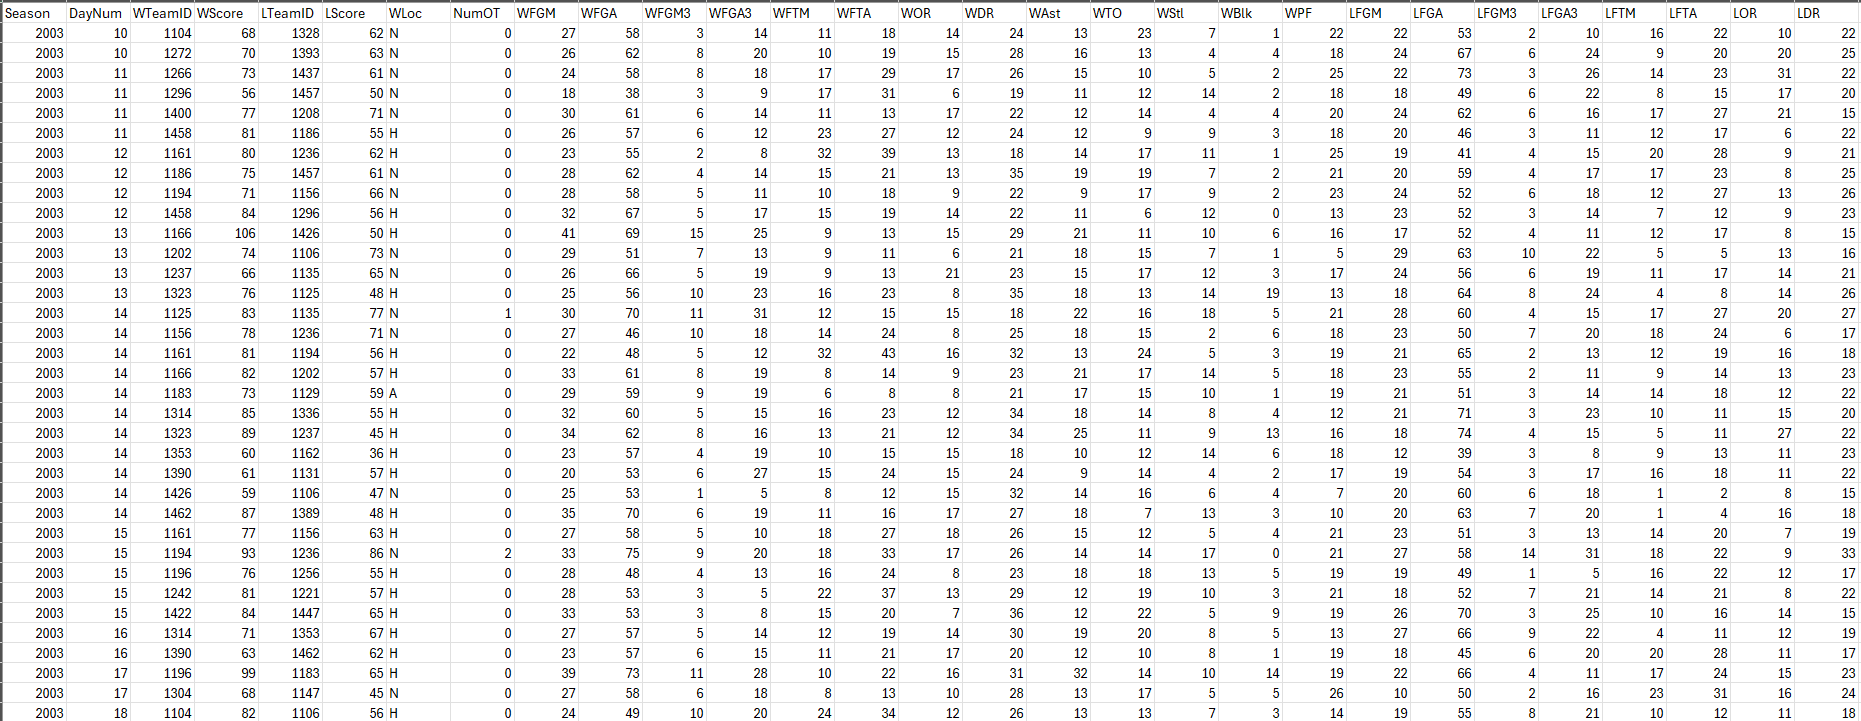
\includegraphics[scale=.3]{paper_photos/regseason.png}
\caption{Regular Season Detailed Data}
\label{regseason}
\end{center}
\end{figure}

This table records key performance metrics for each game played. The schema utilizes the prefix W to denote statistics for the winning team and the prefix L for the losing team. The specific recorded variables include:

\begin{itemize}
    \item Points Scored
    \item The number of field goals made and attempted (FGM-A).
    \item The number of 3-point field goals made and attempted (FGM-A3).
    \item The number of free throws made and attempted (FTM-A).
    \item The number of offensive and defensive rebounds secured (OR- DR).
    \item The number of assists (Ast).
    \item The number of turnovers (TO).
    \item The number of blocks (Blk).
    \item The number of fouls (PF).
\end{itemize}

While raw box scores provide the foundation of events that happened in a game, they often fail to capture nuances in, and out, of the game. To address this limitation, this research supplements the Kaggle datasets with advanced metrics from analyst Ken Pomeroy (KenPom). Pomeroy is accepted as the industry standard for college basketball analysis. Pomeroy's approach is to normalize the data by calculating efficiency rather then raw stats. Theses statistics are updated daily throughout the regular season and tournament. For the purpose of this study, a snapshot of the rankings was acquired from the day prior to the start of the 2025 tournament.  

\begin{figure}[H]
\begin{center}
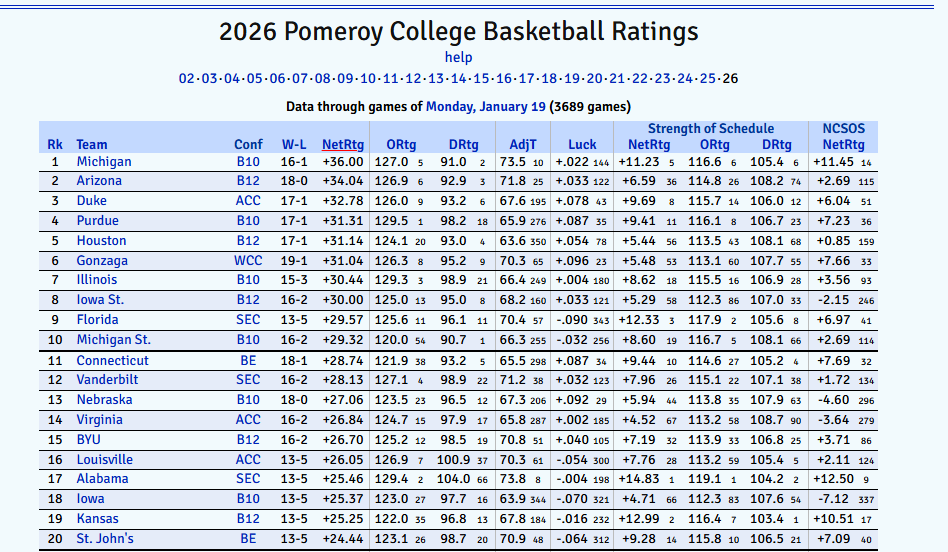
\includegraphics[scale=.5]{paper_photos/kenpom.png}
\caption{The first 20 teams of the KenPom data table.}
\label{kenpom}
\end{center}
\end{figure}

The primary metrics utilized from this source include:
\begin{itemize}
    \item Net Rating (NetRtg).
    \item Offensive Rating (ORtg).
    \item Defensive Rating (DRtg).
    \item Adjusted Tempo (AdjT).
\end{itemize}
Net rating is the differential between Offensive and Defensive Rating. Offensive Rating measures the points scored per $100$ possessions. Similarly, defensive rating measure the points given up per $100$ possessions. These ratings are adjusted by the quality of opponents a team has played, and the game location. Lastly, Adjusted tempo is the number of possessions per $40$ minutes. We define a possession as the period where a team controls the ball, ending with a shot attempt, turnover, or score. 

While Pomeroy's ratings serve as the industry standard, they are exclusively available for the Men's division. Consequently, this research incorporates an additional dataset from Bart Torvik that focuses on the Women's division. Torvik cites Pomeroy as a significant influence; thus, the ratings are constructed using a comparable methodology. However, distinct algorithmic differences exist between the two systems. For further detail regarding these distinctions, the reader is referred to \cite{Torvik}. The metrics used from Barttovik are:
\begin{itemize}
    \item Adjusted Offensive Efficiency (ADJOE).
    \item Adjusted Defensive Efficiency (ADJDE). 
    \item Adjusted Tempo (ADJ T.). 
\end{itemize}

\begin{figure}[H]
\begin{center}
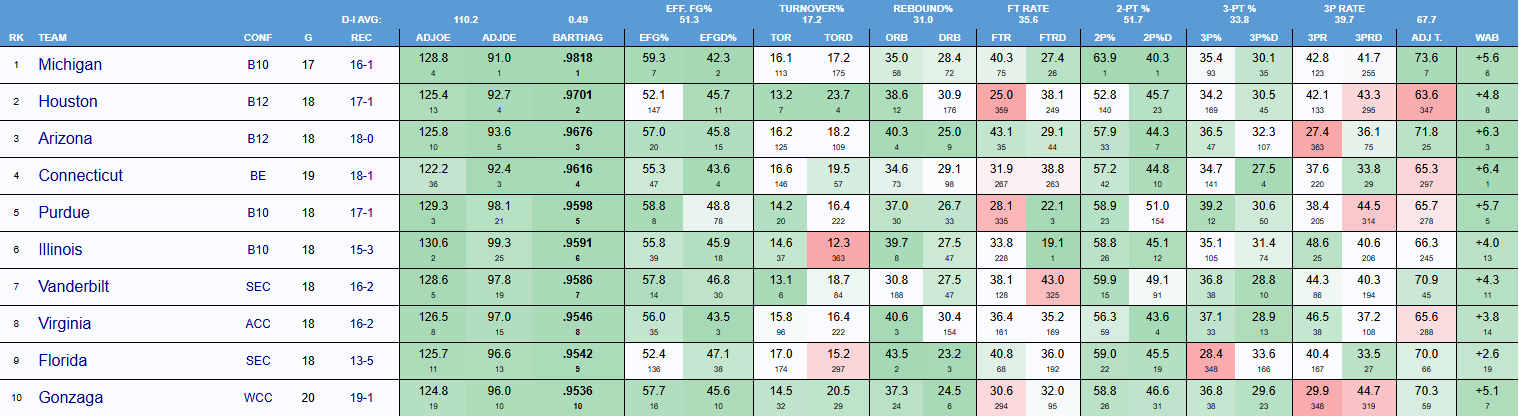
\includegraphics[scale=.35]{paper_photos/bartervik.png}
\caption{The first 10 teams of the Barttorvik table}
\label{barttorvik}
\end{center}
\end{figure}

To complement the efficiency metrics provided by Pomeroy and Torvik, this research also incorporates the comprehensive ranking systems aggregated by Kenneth Massey. While the previously discussed datasets focus on raw predictive efficiency, the Massey Ordinals provide a consolidated view of team hierarchy. This dataset aggregates rankings from over $40$ distinct mathematical systems, pollsters, and algorithms. These rankings typically present data as an ordinal integer where the top team is assigned the value of $1$. Incorporating this data allows the model to leverage a "wisdom of the crowd" approach by utilizing the consensus of the broader analytical community. 

\begin{figure}[H]
\begin{center}
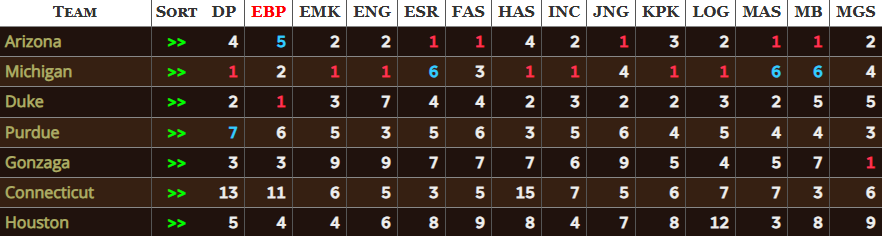
\includegraphics[scale=.5]{paper_photos/massey.png}
\caption{A sample of the Massey Ordinals table showing distinct ranking systems.}
\label{massey}
\end{center}
\end{figure}
One significant challenge in aggregating these distinct sources is the inconsistency in team nomenclature. For instance, a university might be listed as "St. Mary's" in one dataset and "Saint Mary's CA" in another. To resolve this discrepancy, all external data was strictly mapped to the unique TeamID integer provided by the Kaggle competition files. This standardization ensures that the advanced efficiency metrics are accurately merged with the box score data for every specific matchup.



\newpage
%YOU SHOULD USE STANDARD LaTeX TO TYPESET YOUR WORK. USE \ref AND \cite, DO NOT HARDCODE YOUR REFERENCES.


%%%%%%%%%%%%%%%%%%%%%%%%%%






%THIS IS HOW YOU PLACE FIGURES. PLEASE FOLLOW THIS TEMPLATE SO YOUR PICTURES DO NOT FLOAT TO WHERE YOU DO NOT WANT THEM.

%\begin{figure}[H]
%\begin{center}
%\includegraphics[scale=.7]{rw2dn4.pdf}
%\caption{Probability Distribution Frequencies for $n = 4$}
%\label{2dfrequencies}
%\end{center}
%\end{figure}

%%%%%%%%%%%%%%%%%%%%%%%%%%%
%\usubsection{A Third Subsection with an Equation}





%NOTE THAT ABOVE, I FINISHED THE PROOF WITH  \qedhere. THIS IS SO THE SQUARE IS ON THE SAME LINE AS THE LAST LINE WRITTEN. IF YOU COMMENT THAT OUT, YOU WILL SEE THAT THE SQUARE GOES ONE LINE LOWER, UGLY AND BAD PRACTICE.


%%%%%%%%%%%%%%%%%%%%%%%%%%%%%%%%%%%%%%%%%%%%%%%%%%%%%%%%%%%%%%%%
\begin{center}
\section{LITERATURE REVIEW}
\end{center}
\thispagestyle{empty} %NO PAGE NUMBER ON SECTION PAGES.


\usubsection{Past Strategies}
The pursuit of a perfect bracket has generated a substantial body of research in predictive modeling over the last decade. While specific algorithms vary, the most successful strategies in the Kaggle Machine Learning Mania competition consistently rely on one of two distinct methodological frameworks.

The primary objective for this study is to minimize the Brier Score. We define the Brier Score (BS) as follows:

\begin{equation}
    BS = \frac{1}{N} \sum_{t=1}^N (f_t - o_t)^2
\end{equation}

where $N$ is the number of events, $f_t$ is the predicted probability, and $o_t$ is the actual outcome. For this research, a $0$ is considered a loss, and a $1$ is a win. A Brier Score of $0$ would reflect perfect accuracy, while a Brier Score of $1$ reflects perfect inaccuracy. To provide a baseline, a strategy where we predict every team has a $50\%$ chance of winning would result in a Brier Score of $0.25$. (thinking of putting another example here)

The first framework relies on fundamental analysis where the objective is to construct a ground-truth probability independent of public sentiment. A common implementation of this approach involves utilizing domain-specific heuristics such as the elo rating system. Originally designed for chess, elo provides a dynamic measure of team strength that updates after every game. It offers a robust baseline that accounts for strength of schedule more effectively than raw win-loss records \cite{chess}. Many strategies also incorporate expert features. These include the Nate Silver, FiveThirtyEight, and KenPom ratings which act as high-signal inputs that aggregate player health, travel distance, and roster depth into a single numeric value. By treating these expert outputs as features rather than final predictions, modelers can leverage human domain expertise while correcting for known expert biases.

The second dominant framework relies on the Efficient Market Hypothesis \cite{EMH}. This approach posits that global betting markets, specifically closing lines from major bookmakers, offer a more accurate aggregate predictor of game outcomes than individual statistical models. The efficacy of this strategy is well-documented in recent Kaggle competitions where five of the top eight performing models utilized market-derived features as their primary feature. These strategies do not attempt to beat the market. Instead, they focus on mathematically disentangling the true win probability from the bookmaker's overround and inherent biases.

To achieve this, recent state-of-the-art implementations utilize specific conversion algorithms to de-noise betting data. The standard tool in this domain is the $\textit{Goto\_conversion}$. Competitors employ these functions to address the favorite-longshot bias. This is the tendency for markets to overvalue underdogs and undervalue favorites. By applying these corrections, modelers can transform raw Vegas odds into highly calibrated probabilities that minimize Brier Score more effectively than fundamental analysis alone. This approach effectively leverages the crowd wisdom of the market while stripping away the pricing inefficiencies introduced by public betting behavior. For more information on how this strategy works, we refer the reader to \cite{goto}.

The applicability of these methodological frameworks, however, is heavily constrained by the structural discontinuity introduced by the 2021 Name, Image, and Likeness (NIL) legislation. Statistical analysis of the post-NIL landscape reveals a significant deviation from historical norms, characterized by a rapid consolidation of talent where the number of programs with elite win percentages (
$>75\%$) has nearly tripled \cite{CBS}. This phenomenon implies that feature weights derived from pre-2021 eras are likely subject to significant concept drift. Consequently,
this literature review restricts its focus to winning strategies from recent Kaggle competitions (2022-present), as methodologies developed before the NIL era may not reflect the approaches best suited to the heightened stratification of team strength driven by current transfer portal dynamics.
 
\newpage
\usubsection{Modeling Techniques}
Recent tournament prediction methodologies employ several established modeling and computational techniques. This section provides formal definitions for the five core approaches used in this study: Logistic Regression, Linear Regression, Monte Carlo Simulation, Random Forest, and Neural Networks.

Logistic Regression is a binary classification model that estimates the probability of an outcome by applying the logistic (also known as sigmoid) function to a linear combination of input features. The model is defined as:

\begin{equation}
P(Y=1|X) = \frac{1}{1 + e^{-(\beta_0 + \beta_1 x_1 + \beta_2 x_2 + ... + \beta_n x_n)}}
\end{equation}
where $Y$ is the binary outcome, $X = (x_1,x_2,\ldots,x_n)$ represents the feature vector, and $\beta = (\beta_0,\beta_1\, \ldots, \beta_n)$ are the model coefficients estimated through the maximum likelihood estimation. This function ensures the predicted probabilities are bounded between $[0,1]$. Logistic regression assumes a linear relationship between the input features and the log-odds of the outcome. This assumption can be restrictive when the true relationships are nonlinear. To address this limitation, common approaches are feature engineering with polynomial or interaction terms (e.g, $x^2, x_i \cdot x_j)$ to capture nonlinear patterns. 

Linear Regression is a supervised learning method that models the relationship between a dependent variable and one or more independent variables by fitting a linear equation to the observed data. Linear Regression is defined as:

\begin{equation}
\hat{Y} = \beta_0 + \beta_1 x_1 + \beta_2 x_2 + \ldots + \beta_n x_n
\end{equation}
where $\hat{Y}$ is the predicted continuous outcome, $X = (x_1, x_2, \ldots, x_n)$ represents the vector of features, and $\beta = (\beta_0, \beta_1, \ldots, \beta_n)$ are the model coefficients estimated through ordinary least squares (OLS) minimization. For more information on OLS we refer the reader to \cite{OLS}. Unlike logistic regression, linear regression produces unbounded predictions and does not inherently output probabilities. In sports prediction contexts, linear regression is commonly used to estimate point totals, scoring margins, or other continuous performance metrics that can subsequently be transformed into win probabilities through additional techniques.

\begin{figure}[H]
    \centering
    % First Figure
    \begin{minipage}{0.45\textwidth}
        \centering
        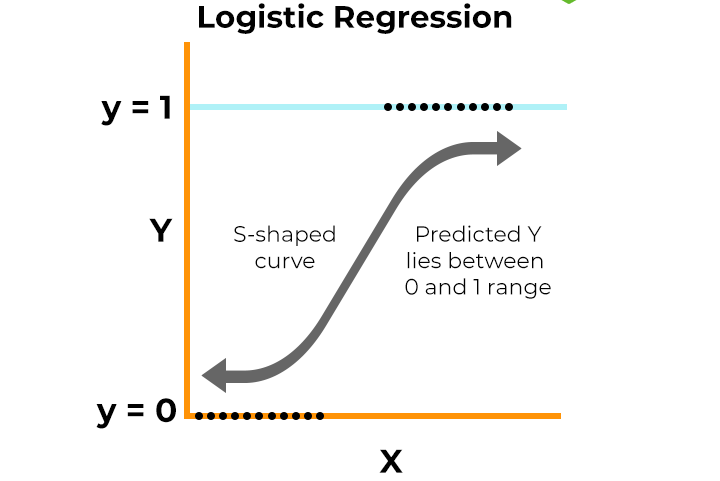
\includegraphics[width=\linewidth]{paper_photos/logisticreg.png}
        \caption{An Example of a Logistic Regression Equation \cite{logphoto}.}
        \label{logistic}
    \end{minipage}\hfill
    % Second Figure
    \begin{minipage}{0.45\textwidth}
        \centering
        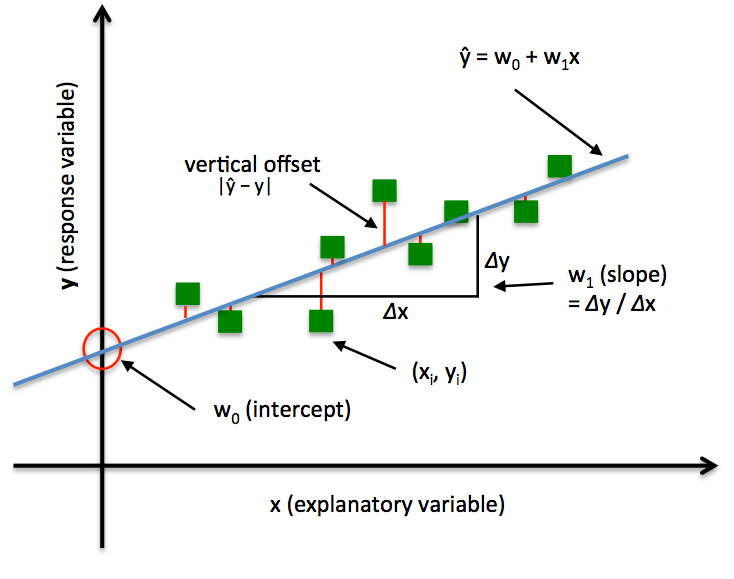
\includegraphics[width=\linewidth]{paper_photos/simple_regression.png}
        \caption{An Example of a Linear Regression Equation \cite{linearphoto}.}
        \label{linear}
    \end{minipage}
\end{figure}

Monte Carlo Simulation is a computational technique that uses repeated random sampling to estimate probabilities for systems with inherent uncertainty. The method generates $N$ independent samples $x_1, x_2, \ldots, x_N$ from a probability distribution $f(x)$, then estimates probabilities by computation the proportion of samples satisfying a certain condition. The simulation is defined as:
\begin{equation}
\hat{P} = \frac{1}{N}\sum_{i=1}^{N} {1}(x_i \in A)
\end{equation}
where $1(\cdot)$ is the indicator function that equals $1$ when the condition is satisfied and $0$ otherwise. $A$ represents the event of interest, and $\hat{P}$ is the Monte Carlo estimate of the true probability $P(A)$. By the Law of Large Numbers \cite{Large Numbers}, $\hat{P} \to P(A)$ as $N \to \infty$. In sports prediction contexts, Monte Carlo methods are frequently employed to simulate game outcomes by sampling from estimated score distributions, enabling the estimation of win probabilities through empirical frequency counts across simulated matchups.

XGBoost (Extreme Gradient Boosting), considered a "black-box" approach, is an ensemble learning method that constructs a sequence of decision trees where each successive tree is trained to correct the residual errors of the previous trees. Unlike Random Forest, which builds trees independently, XGBoost employs gradient boosting to iteratively minimize a loss function through additive modeling \cite{XGBoost}. The model prediction is defined as the sum of predictions from all trees:
\begin{equation}
\hat{y}_i = \sum_{k=1}^K f_k(x_i).
\end{equation} 
Here, $f_k(x_i)$ is the prediction of the $k^{\text{th}}$ tree for the $i^{\text{ith}}$ data point, $\hat{y}_i$ is the final predicted value for the  $i^{\text{ith}}$ data point, and $K$ is the number of trees. Each tree is trained to minimize the objective function 

\begin{equation}
    \text{obj}(\theta) = \sum_{i}^n l(y_i, \hat{y}_i) + \sum_{k=1}^K \Omega(f_k)
\end{equation}
where $l$ is the loss function which simply computes the difference between the true and predicted, and $\Omega$ is the regularization term, discouraging overly complex trees. The optimization process then proceeds via gradient descent on the residuals. For more information regarding gradient descent we refer the reader to \cite{GD}. XGBoost is widely adopted in competitive machine learning for its performance on structured data and ability to capture complex interactions and relationships between features. 

\begin{equation}
h^{(\ell)} = \sigma\left(W^{(\ell)} h^{(\ell-1)} + b^{(\ell)}\right)
\end{equation}
if i do neural nets i will keep going with this. 
\newpage

%%%%%%%%%%%%%%%%%%%%%%%%%%%%%%%%%%%%%%%%%%%%%%%%%%%%%%%%%%%%%%%%
\begin{center}
\section{Probability Prediction Models}
\end{center}
\thispagestyle{empty} %NO PAGE NUMBER ON SECTION PAGES.
This section details the development and evaluation of models designed to predict a continuous win probability $P \in (0, 1)$ for any given matchup.  While the tournament results are ultimately binary, the Brier Score evaluation metric heavily penalizes overconfidence in incorrect predictions and rewards well-calibrated probabilities. Consequently, this research moves beyond simple classification to focus on models that quantify the uncertainty inherent in the March Madness environment. By establishing a framework where a value $P > 0.5$ denotes a predicted victory for Team A, a baseline is created for performance that accounts for the high variance of single-elimination play. This probabilistic approach serves as the engine of the project and bridges the gap between theoretical literature and the empirical application of machine learning.

To expand further on these concepts, the methodology begins with a rigorous data processing phase where historical box scores are transformed into a symmetric training set.  This ensures that the models learn to evaluate the relative strength between two competitors rather than relying on arbitrary formatting artifacts. This section details the complete machine learning pipeline implemented for the 2026 tournament prediction. We first examine the data cleaning procedures required to tailor the feature sets to the specific statistical assumptions of each algorithm. Following this, we explore the variable selection process used to identify high signal metrics such as KenPom and Massey data. Finally, we implement and compare two distinct modeling architectures, specifically Logistic Regression and XGBoost, to determine which approach best minimizes the Brier Score in a high variance environment.

\usubsection{Logistic Regression}
\usubsubsection{Variable Selection}
To accurately model basketball outcomes, one must first deconstruct the sport into its atomic statistical events. A standard game is composed of a finite sequence of possessions. Within these possessions, specific discrete actions determine the flow of the contest. The primary events recorded in the raw dataset include Field Goals, Free Throws, Rebounds, Turnovers, and Personal Fouls. A Field Goal ($FGM$) represents the primary method of scoring and is worth either two or three points. A Free Throw ($FTM$) is an unopposed attempt worth one point awarded after a foul. A Rebound is recorded when a player retrieves the ball after a missed shot; this is further categorized into Offensive Rebounds ($OR$), which grant the shooting team a second opportunity, and Defensive Rebounds ($DR$), which terminate the opponent's possession. Finally, a Turnover ($TO$) is a loss of possession due to a violation or steal, resulting in zero points.

Analyzing these events using raw totals is statistically flawed due to the confounding variable of pace. A team that plays at a high tempo may record high totals for points and rebounds simply because they generate more possessions, not because they are efficient. To resolve this, this model utilizes the "Four Factors of Basketball Success." Developed by Dean Oliver, this framework isolates the four specific components that correlate most strongly with winning: shooting efficiency, turnover avoidance, rebounding dominance, and free throw frequency \cite{Dean}. 

Crucial to these efficiency calculations is the estimation of total Possessions ($Poss$). A possession is defined as the period during which a team controls the ball, ending with a shot attempt, a turnover, or a trip to the free-throw line.  Since possessions are not explicitly tracked in standard box scores, they must be estimated using the following formula: \begin{equation}Poss = (FGA - OR) + TO + (0.44 \cdot FTA).\end{equation}

This equation aggregates the three ways a possession can end: a field goal attempt ($FGA$), a turnover ($TO$), or free throws ($FTA$). The term $(FGA - OR)$ accounts for missed shots that are rebounded by the offense; because the team retains the ball, the possession continues, and thus the initial attempt is subtracted to avoid double-counting. The coefficient $0.44$ applied to Free Throw Attempts estimates the proportion of trips to the line that actually terminate a possession (e.g., the second of two shots), accounting for and-one (fouled while successfully scoring) situations and technical fouls. This derived metric serves as the denominator for rate statistics, allowing for a direct comparison between teams of differing tempos.

The first factor is Effective Field Goal Percentage ($eFG\%$). This metric refines standard field goal percentage by accounting for the fact that a three-point shot is worth $50\%$ more than a two-point shot. It is calculated as:
\begin{equation}
eFG\% = \frac{FGM + 0.5 \cdot FGM3}{FGA}
\end{equation}
By including the $0.5$ weighting for three-pointers ($FGM3$), this variable measures a team's ability to maximize points per attempt regardless of their shot selection strategy.
The second factor is Turnover Percentage ($TOV\%$). Unlike raw turnover counts, this metric normalizes errors against the total number of possessions calculated above.
\begin{equation}
TOV\% = \frac{TO}{Poss}
\end{equation}
This ratio identifies teams that value the basketball. A lower percentage indicates a disciplined offense that rarely forfeits scoring opportunities.
The third factor is Offensive Rebound Percentage ($ORB\%$). This metric measures a team's physical dominancr relative to their available opportunities. Using raw offensive rebound totals is misleading because a team that misses many shots will naturally have more chances to rebound. This metric corrects for that bias by comparing offensive rebounds ($OR$) to the total number of rebounds available at that specific rim:
\begin{equation}
ORB\% = \frac{OR}{OR + DR_{opp}}
\end{equation}
Here, $DR_{opp}$ represents the defensive rebounds secured by the opponent. A higher percentage indicates a team that frequently generates "second chance" points.
Finally, the model incorporates Win Percentage ($Win\%$) as a fifth feature to capture intangible qualities such as coaching and clutch performance. This is calculated as the mean of the binary game results ($1$ for a win, $0$ for a loss) over the course of the season. Crucially, the logistic regression algorithm does not process these values in isolation. Instead, the dataset is transformed to calculate the differential between the two competing teams for every metric (e.g., $eFG\%_{diff} = eFG\%_{TeamA} - eFG\%_{TeamB}$). This centers the analysis on the relative mismatch between the opponents rather than their absolute statistics.

\usubsubsection{Data Cleaning}

To construct a robust predictive pipeline, the data architecture must establish a strict boundary between feature generation and model training. The independent variables, specifically the Four Factors and Win Percentage, are calculated exclusively utilizing historical regular-season detailed results. Conversely, the logistic regression algorithm is trained entirely on historical NCAA tournament outcomes. By isolating regular-season efficiency metrics as the predictors and tournament game results as the target variable, the framework ensures that the model evaluates how a team's sustained performance over a thirty-game span translates to the high-variance, single-elimination environment of postseason play. This distinction is critical, as regular-season data provides a sufficiently large sample size to stabilize efficiency metrics, while tournament data provides the specific contextual outcomes the model ultimately aims to predict.

Furthermore, to prevent data leakage and simulate the exact informational constraints of a real-world forecaster, the logistic regression model is trained using a strictly defined rolling time window. To evaluate historical accuracy and construct valid out-of-sample predictions, the framework is systematically back tested across consecutive tournament years. For example, to generate probability forecasts for the 2025 NCAA Tournament, the model is trained exclusively on the tournament matchups from the preceding 2023 and 2024 seasons. The decision to restrict the training data to a brief temporal window is grounded in the structural realities of collegiate athletics. NCAA basketball is characterized by high roster turnover, as student-athletes possess limited eligibility and typically serve as primary contributors for only three to four seasons. Consequently, a university program undergoes a complete personnel and strategic transformation within a short cycle. Training the algorithm on data exceeding this window would introduce noise from past iterations of a team that share no roster overlap with the current squad. During this localized training phase, the algorithm maps the recent regular-season metrics to their respective tournament results, learning the optimal coefficient weights without accessing any data from the target prediction year. This rolling training window shifts iteratively for historical benchmark predictions, ensuring that all evaluations remain mathematically rigorous and entirely devoid of look-ahead bias.

The primary obstacle in processing the historical game records is the fundamental structure of the Kaggle dataset. The raw regular-season and tournament data files utilize a deterministic outcome schema. Within this structure, every game observation is explicitly bifurcated into winning and losing statistics. Metrics belonging to the victorious program are assigned column headers prefixed with a 'W', while the defeated opponent's metrics are prefixed with an 'L'.

If a classification algorithm is trained directly on this format, it inevitably suffers from severe target leakage. The logistic regression algorithm would trivially learn to associate the column position with the outcome, mathematically recognizing that the entity occupying the 'W' feature space possesses a 100 percent win probability. This renders the model entirely incapable of out-of-sample prediction, as the ultimate objective is to forecast matchups between two neutral entities before the outcome is known. The following output illustrates this problematic data architecture, demonstrating how the game result is inherently encoded into the feature presentation itself.

\begin{table}[h!]
\begin{knitrout}
\definecolor{shadecolor}{rgb}{0.969, 0.969, 0.969}\color{fgcolor}\begin{kframe}
\begin{alltt}
\hlkwd{head}\hldef{(mens_results} \hlopt{%>%}
       \hlkwd{select}\hldef{(Season, WTeamID, WScore,}
              \hldef{LTeamID, LScore, WFGM,}
              \hldef{LFGM, WTO, LTO),} \hlnum{4}\hldef{)}
\end{alltt}
\begin{verbatim}
##    Season WTeamID WScore LTeamID LScore  WFGM  LFGM   WTO   LTO
##     <int>   <int>  <int>   <int>  <int> <int> <int> <int> <int>
## 1:   2003    1104     68    1328     62    27    22    23    18
## 2:   2003    1272     70    1393     63    26    24    13    12
## 3:   2003    1266     73    1437     61    24    22    10    12
## 4:   2003    1296     56    1457     50    18    18    12    19
\end{verbatim}
\end{kframe}
\end{knitrout}
\caption{Snapshot of raw Kaggle regular-season data demonstrating the 'W' and 'L' column structure.}
  \label{tab:raw_data}
\end{table}


To resolve the target leakage inherent in the raw dataset, the first phase of data processing transforms the game-level observations into season-level team averages. This transformation is executed via the \texttt{calculate\_four\_factors} function. Initially, the function estimates the total possessions for both the winning and losing teams using the standard formula. Subsequently, it computes the Four Factors (Effective Field Goal Percentage, Turnover Percentage, Offensive Rebound Percentage, and Free Throw Rate) for each team in every game.

Rather than maintaining the winner and loser statistics in a single row, the function separates the victors and the defeated into two distinct dataframes. A binary \texttt{Win} variable is appended, assigning a value of $1$ to the winning dataframe and $0$ to the losing dataframe. These two structures are then vertically concatenated using a row-bind operation. Finally, the data is grouped by \texttt{Season} and \texttt{TeamID} to calculate the mean of all numeric variables. This yields a single, stable efficiency profile and an aggregate regular season win percentage for every program in a given year.

\begin{knitrout}
\definecolor{shadecolor}{rgb}{0.969, 0.969, 0.969}\color{fgcolor}\begin{kframe}
\begin{alltt}
\hldef{prepare_model_data} \hlkwb{<-} \hlkwa{function}\hldef{(}\hlkwc{tourney_results_df}\hldef{,}
                               \hlkwc{four_factors_df}\hldef{) \{}

\hldef{training_data} \hlkwb{<-} \hldef{tourney_results_df} \hlopt{%>%}
\hlkwd{mutate}\hldef{(}
\hlkwc{Team1} \hldef{=} \hlkwd{pmin}\hldef{(WTeamID, LTeamID),}
\hlkwc{Team2} \hldef{=} \hlkwd{pmax}\hldef{(WTeamID, LTeamID),}
\hlkwc{Team1_win} \hldef{=} \hlkwd{if_else}\hldef{(Team1} \hlopt{==} \hldef{WTeamID,} \hlnum{1}\hldef{,} \hlnum{0}\hldef{)}
\hldef{)} \hlopt{%>%}
\hlkwd{select}\hldef{(Season, Team1, Team2, Team1_win)}

\hldef{model_data} \hlkwb{<-} \hldef{training_data} \hlopt{%>%}
\hlkwd{left_join}\hldef{(four_factors_df,}
          \hlkwc{by} \hldef{=} \hlkwd{c}\hldef{(}\hlsng{"Season"}\hldef{,} \hlsng{"Team1"} \hldef{=} \hlsng{"TeamID"}\hldef{))} \hlopt{%>%}
\hlkwd{rename_with}\hldef{(}\hlopt{~}\hlkwd{paste0}\hldef{(.,} \hlsng{"_T1"}\hldef{),}
\hlkwc{.cols} \hldef{=} \hlopt{-}\hlkwd{c}\hldef{(Season, Team1, Team2, Team1_win))} \hlopt{%>%}
\hlkwd{left_join}\hldef{(four_factors_df,}
          \hlkwc{by} \hldef{=} \hlkwd{c}\hldef{(}\hlsng{"Season"}\hldef{,} \hlsng{"Team2"} \hldef{=} \hlsng{"TeamID"}\hldef{))} \hlopt{%>%}
\hlkwd{rename_with}\hldef{(}\hlopt{~}\hlkwd{paste0}\hldef{(.,} \hlsng{"_T2"}\hldef{),}
\hlkwc{.cols} \hldef{=} \hlopt{-}\hlkwd{c}\hldef{(Season, Team1, Team2, Team1_win,} \hlkwd{ends_with}\hldef{(}\hlsng{"_T1"}\hldef{)))} \hlopt{%>%}
\hlkwd{mutate}\hldef{(}
\hlkwc{eFG_diff}     \hldef{= eFG_T1} \hlopt{-} \hldef{eFG_T2,}
\hlkwc{TOV_Pct_diff} \hldef{= TOV_Pct_T1} \hlopt{-} \hldef{TOV_Pct_T2,}
\hlkwc{ORB_Pct_diff} \hldef{= ORB_Pct_T1} \hlopt{-} \hldef{ORB_Pct_T2,}
\hlkwc{FTR_diff}     \hldef{= FTR_T1} \hlopt{-} \hldef{FTR_T2,}
\hlkwc{Win_diff}     \hldef{= Win_T1} \hlopt{-} \hldef{Win_T2}
\hldef{)} \hlopt{%>%}
\hlkwd{na.omit}\hldef{()}

\hlkwd{return}\hldef{(model_data)}
\hldef{\}}
\end{alltt}
\end{kframe}
\end{knitrout}

\usubsubsection{Model Implementation}

Following the systematic cleaning and neutralization of the dataset, the analysis proceeds to the implementation of the predictive framework. The primary objective is to construct a logistic regression pipeline capable of generating calibrated win probabilities for every possible matchup in the 2026 NCAA Tournament. This method is chosen specifically for its ability to model the probability of a binary outcome, in this case whether the lower-ID team (Team 1) wins or loses, based on a linear combination of statistical differentials. The models utilize a logit link function to map the relationship between the independent variables and the probability of a victory. The formal specification for each model iteration is defined by the following equation:

\begin{equation}
\begin{split}
\text{logit}(P) = \ln\left(\frac{P}{1-P}\right) = \beta_0 & + \beta_1(\text{eFG\_diff}) + \beta_2(\text{TOV\_diff}) \\
& + \beta_3(\text{ORB\_diff}) + \beta_4(\text{FTR\_diff}) + \beta_5(\text{Win\_diff})
\end{split}
\end{equation}

Where $P$ represents the probability of a Team 1 victory. The coefficients ($\beta$) represent the change in log-odds of winning for every one unit increase in the respective statistical differential.

The model is estimated using maximum likelihood estimation, which identifies the coefficient vector $\beta$ that maximizes the probability of observing the recorded tournament outcomes given the input differentials. Because the response variable is binary, the log-likelihood function takes the form:

\begin{equation}
\sum_{i=1}^n \left[ y_i \log p(x_i) + (1-y_i)\log(1-p(x_i)) \right]
\end{equation}

where $y_i \in \{0, 1\}$ is the observed outcome for the $i$-th matchup and $p(x_i)$ is the model's predicted probability \cite{logistic} of a Team 1 victory. Maximizing this function is equivalent to minimizing the binary cross-entropy loss. The resulting coefficients reflect both the direction and magnitude of each differential's contribution to the probability of winning. A positive coefficient on \texttt{eFG\_diff}, for instance, indicates that a larger shooting efficiency advantage is associated with a higher probability of victory, which is consistent with what basketball theory would predict.

For the 2026 deployment, separate models are trained for the men's and women's divisions. The choice to train independent models for each division rather than a single combined model with a gender indicator reflects a fundamental assumption that the Four Factors carry structurally different predictive weight in the men's and women's game. Differences in pace, physicality, and three-point volume between the two divisions suggest that the relationship between shooting efficiency and winning probability may not be uniform across genders. Training separate models allows each set of coefficients to reflect the unique dynamics of its respective division rather than forcing a shared parameter estimate that could mask meaningful differences. 

Nonetheless, Each model is trained exclusively on tournament outcomes from the 2024 and 2025 seasons, with the corresponding regular-season Four Factors serving as the independent variables. This two-year window was selected to reflect the current competitive landscape of college basketball while respecting the structural roster turnover discussed previously. The Kaggle competition provides a submission file containing every possible 2026 tournament matchup, numbering in the thousands of pairings across both divisions. The Four Factors for each team are computed from their 2025 regular-season results and differenced for every candidate pairing. The fitted models then generate a probability $\hat{P} \in (0,1)$ for each of these matchups via the inverse logit transformation, producing the final submission.

An important practical consideration in this implementation is the relatively small sample size introduced by the two-year training window. A single NCAA tournament produces only 63 games for the men's bracket and 63 for the women's, yielding a combined training pool of roughly 250 observations per model iteration. While this is sufficient for a low-dimensional model such as logistic regression, it places meaningful constraints on the complexity of the architecture that can be reliably estimated. Overfitting becomes a nontrivial risk if additional interaction terms or polynomial features are introduced without sufficient regularization. For this reason, the model is deliberately kept simple, relying on five theoretically motivated differentials rather than a broader set of engineered features. This simplicity is consistent with the principle of Occam's Razor in model selection \cite{occam}, where a simpler model that generalizes well out-of-sample is preferred over a complex one that fits the training data too closely.

Prior to submitting predictions for the 2026 tournament, the pipeline is validated through a series of backtests spanning the 2023, 2024, and 2025 competitions. These historical evaluations serve a specific purpose: to confirm that the rolling two-year training window generalizes to unseen tournament data before any live predictions are committed. For the 2023 backtest, the model is trained on tournament outcomes from 2021 and 2022. For the 2024 backtest, the training window shifts forward to include 2022 and 2023. Finally, for the 2025 backtest, the model is trained on 2023 and 2024 tournament data. In each case, the Four Factors are derived exclusively from the regular-season data preceding the target year, and no tournament results from the prediction year are ever introduced into the training process.

The resulting Brier Scores from these backtests are compared against the winning submission scores published by Kaggle for the corresponding competition years. This comparison provides a meaningful external benchmark, situating the logistic regression framework within the broader landscape of competitor strategies. Table \ref{tab:brier_results} summarizes the Brier Scores produced by the model across all three backtest years alongside the winning scores for their respective competitions.

\begin{table}[h!]
\centering
\caption{Logistic Regression Backtest Results vs. Kaggle Benchmarks}
\label{tab:brier_results}
\begin{tabular}{lcc}
\hline
\textbf{Tournament Year} & \textbf{Model Brier Score} & \textbf{Winning Brier Score} \\ \hline
2023 & 0.21653 & 0.17371 \\
2024 & 0.21064 & 0.05313 \\
2025 & 0.18401 & 0.10411 \\ \hline
\end{tabular}
\end{table}

It is important to note that the 2024 winning Brier Score of 0.05313 is not directly comparable to the scores recorded in 2023 and 2025. In that competition year, Kaggle introduced a significant structural change to the submission format. Rather than submitting a single set of game-by-game win probabilities, competitors were permitted to submit a portfolio of up to one hundred thousand distinct bracket entries. The final score was then computed by averaging the Brier Score across rounds rather than across individual games, placing substantially greater weight on later-round matchups where fewer games are played. This round-weighted averaging mechanism naturally compresses scores toward lower values relative to the standard per-game formulation. Consequently, the 0.05313 figure reflects a fundamentally different evaluation environment and should be interpreted as a benchmark specific to the 2024 format rather than as evidence of superior predictive accuracy over other competition years.

Setting aside the 2024 anomaly, the remaining backtests reveal a consistent trend of improvement. The model's Brier Score declined from 0.21653 in 2023 to 0.18401 in 2025, reflecting incremental gains in calibration as the pipeline was refined. Crucially, the 2025 backtest represents the most direct analog to the 2026 submission, as it uses the identical training structure and feature set that will be deployed. While the model trails the top competitors in each year, it remains well above the naive 0.25 baseline and demonstrates stable generalization across multiple tournament cycles. These results provided sufficient confidence in the pipeline to justify its deployment for the 2026 Kaggle submission.

\usubsubsection{Model Analysis}
With the models estimated on the 2023 and 2024 tournament data, the resulting coefficients can be examined to evaluate which of the Four Factors carry meaningful predictive weight in each division. Because separate models were trained for the men's and women's tournaments, the coefficient structures can be analyzed independently and then compared to assess whether the Four Factors operate differently across divisions. Tables \ref{tab:mens_coef} and \ref{tab:womens_coef} present the estimated coefficients, p-values, and significance levels for the men's and women's models respectively.

% latex table generated in R 4.4.2 by xtable 1.8-4 package
% Mon Mar  9 23:12:36 2026
\begin{table}[ht]
\centering
\caption{Logistic Regression Coefficient Estimates (Men's 2025 Model)} 
\label{tab:mens_coef}
\begin{tabular}{lrrl}
  \hline
Variable & Estimate & p-value & Sig. \\ 
  \hline
Intercept & 0.4352 & 0.0348 & * \\ 
  eFG Diff & 7.7952 & 0.2244 &  \\ 
  TOV Pct Diff & -20.5106 & 0.0901 & . \\ 
  ORB Pct Diff & 12.3634 & 0.0027 & ** \\ 
  FTR Diff & -1.4307 & 0.7527 &  \\ 
  Win Diff & 1.3253 & 0.4365 &  \\ 
   \hline
\end{tabular}
\end{table}
% latex table generated in R 4.4.2 by xtable 1.8-4 package
% Mon Mar  9 23:12:36 2026
\begin{table}[ht]
\centering
\caption{Logistic Regression Coefficient Estimates (Women's 2025 Model)} 
\label{tab:womens_coef}
\begin{tabular}{lrrl}
  \hline
Variable & Estimate & p-value & Sig. \\ 
  \hline
Intercept & -0.0888 & 0.6657 &  \\ 
  eFG Diff & 17.4458 & 0.0016 & ** \\ 
  TOV Pct Diff & -19.8212 & 0.0237 & * \\ 
  ORB Pct Diff & 12.4308 & 0.0004 & *** \\ 
  FTR Diff & 3.9742 & 0.4420 &  \\ 
  Win Diff & -1.8468 & 0.4172 &  \\ 
   \hline
\end{tabular}
\end{table}


In the men's model, the only variable to reach conventional statistical significance is Offensive Rebound Percentage, with an estimated coefficient of 12.3634 and a p-value of 0.003. The positive sign is theoretically consistent with Dean Oliver's framework \cite{Dean}, as a team that dominates the offensive glass generates additional possessions while simultaneously denying the opponent easy transition opportunities. Turnover Percentage approaches significance at the 0.10 level with an estimate of -20.5106, and the negative direction is again theoretically correct, as a team that surrenders possessions more frequently than its opponent is expected to win less often. Effective Field Goal Percentage, Free Throw Rate, and Win Percentage all fail to reach significance in the men's model, suggesting that within the narrow two-year training window, shooting efficiency differentials and win records carry limited additional explanatory power once rebounding and turnover control are accounted for. The intercept of 0.4352 is statistically significant at the 0.05 level, implying a slight structural tendency for the lower-ID team to win in the men's tournament even after controlling for all efficiency differentials. This is likely an artifact of the team ID assignment convention rather than a genuine basketball phenomenon.

The women's model tells a different story. Three variables reach statistical significance: Offensive Rebound Percentage (12.4308, $p < 0.001$), Effective Field Goal Percentage (17.4458, $p = 0.002$), and Turnover Percentage (-19.8212, $p = 0.024$). The consistency of Offensive Rebound Percentage across both models is the single most robust finding of this analysis, as the near identical magnitude of the estimates (12.36 in the men's model and 12.43 in the women's model) across two independently trained models strongly suggests that second chance scoring dominance is a universal determinant of tournament success regardless of division. The women's intercept is effectively zero and insignificant, indicating no structural bias toward either team ordering in that division.

The most substantive structural difference between the two models is the role of Effective Field Goal Percentage. In the women's model, it is the second most significant predictor with a coefficient nearly twice the magnitude of the men's estimate. In the men's model, the same variable is statistically indistinguishable from zero. This divergence suggests that shooting efficiency differentials are a more decisive factor in women's tournament outcomes, where a meaningful gap in $eFG\%$ between two opponents translates more reliably into a victory. In the men's tournament, the compressed talent distribution and faster pace of play may reduce the marginal impact of a given efficiency advantage, as superior athleticism and shot creation ability can compensate for efficiency deficits in ways that are not captured by the Four Factors alone. This finding provides direct empirical support for the decision to train the two models independently rather than pooling them under a shared parameter structure. Had a combined model been used, the women's strong shooting efficiency signal would have been diluted by the men's null result, and the men's rebound signal would have been the only surviving predictor across both divisions.

Free Throw Rate fails to reach significance in either model, which is consistent with the nature of the statistic itself. Unlike shooting efficiency or turnover rate, free throw volume tends to be relatively stable across teams at the tournament level, as elite programs generally reach the line at comparable rates. When the differential between two opponents is consistently narrow, the variable carries little discriminatory power and the model appropriately assigns it a negligible coefficient. Win Percentage similarly contributes no significant explanatory power in either model once the efficiency differentials are controlled for. This suggests that the Four Factors effectively subsume the information contained in raw win-loss records; a team's season-long efficiency profile captures the underlying quality of the program more precisely than its aggregate record, which can be inflated or deflated by schedule strength and margin of victory.

\usubsubsection{Results}

The performance of the 2025 logistic regression models is evaluated along two dimensions: classification accuracy via the confusion matrices and probability calibration via the Brier Score. Figure \ref{fig:conf_matrices_2025} presents the confusion matrices for the men's, women's, and combined models.

\begin{knitrout}
\definecolor{shadecolor}{rgb}{0.969, 0.969, 0.969}\color{fgcolor}\begin{figure}
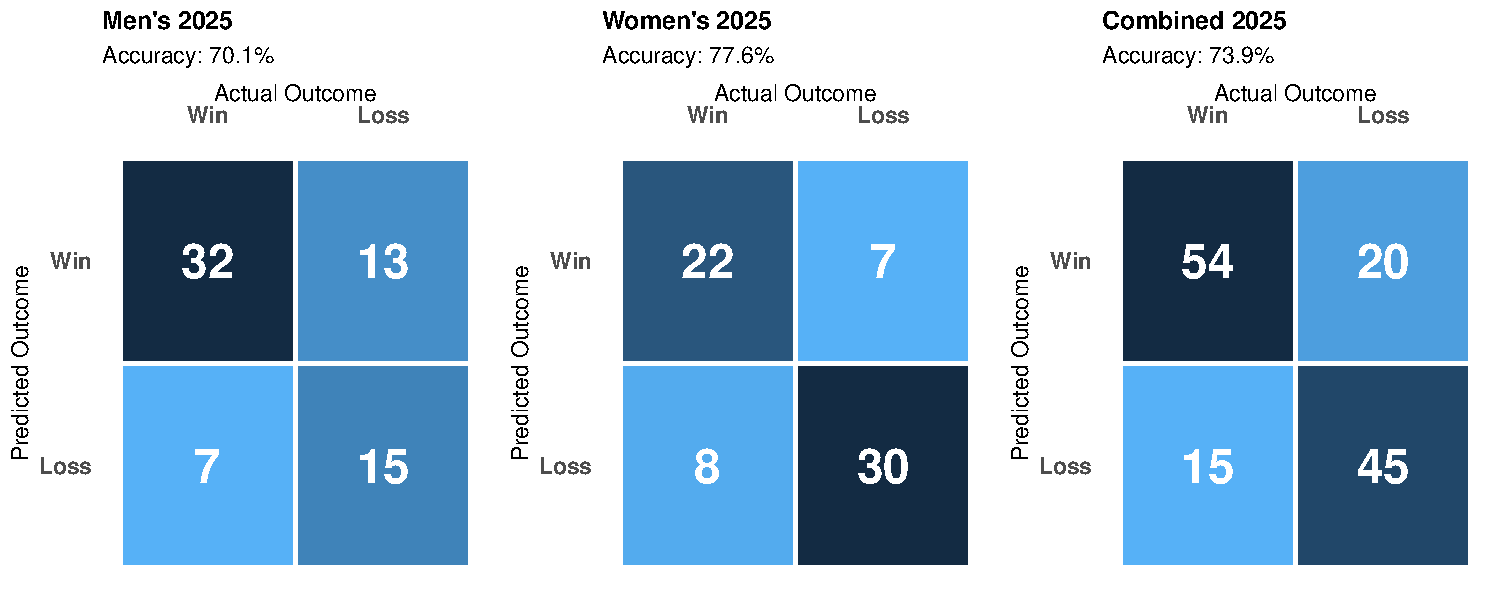
\includegraphics[width=\textwidth]{figure/conf_matrices_2025-1} \caption[Confusion Matrices for the 2025 Logistic Regression Models]{Confusion Matrices for the 2025 Logistic Regression Models}\label{fig:conf_matrices_2025}
\end{figure}

\end{knitrout}

The women's model achieves the strongest classification performance at 77.6\% accuracy, followed by the combined model at $73.9\%$ and the men's model at $70.1\%$. This ordering is consistent with the coefficient analysis in the prior section. The women's model benefits from three statistically significant predictors, Offensive Rebound Percentage, Effective Field Goal Percentage, and Turnover Percentage, providing a richer signal for binary classification. The men's model, where only Offensive Rebound Percentage reaches conventional significance, has a narrower basis for discrimination and consequently misclassifies a greater proportion of games. All three accuracy figures comfortably exceed the $50\%$ baseline that would be expected from random prediction, indicating that the Four Factors carry genuine discriminatory power in both divisions.

However, classification accuracy alone is an incomplete measure of model quality in this context. The Brier Score evaluation framework penalizes not just incorrect predictions but overconfident ones, meaning a model that correctly identifies the winner but assigns a probability of 0.95 rather than $0.65$ is still penalized heavily when upsets occur. The combined 2025 Brier Score of $0.18401$ reflects this tension. While the model demonstrates solid directional accuracy, the gap between its Brier Score and the competition winning score of $0.10411$ suggests that the predicted probabilities are not as well calibrated as those produced by the top competitors. This is an expected limitation of a parsimonious four factor framework. Models that incorporate additional signals such as KenPom efficiency ratings, seed differentials, or market-derived probabilities are better positioned to assign more conservative probabilities to matchups involving significant uncertainty, which is precisely where the Brier Score penalizes most heavily.

Despite this gap, the 2025 results validate the pipeline as a functional and reproducible baseline. The model generalizes consistently across both divisions, produces accuracy well above chance, and maintains a Brier Score substantially below the naive $0.25$ baseline. These characteristics provide a foundation from which the more sophisticated modeling techniques discussed in the following sections aim to improve.

%%%%%%%%%%%%%%%%%%%%%%
\newpage
\usubsection{Boosting}
While logistic regression provides an interpretable and theoretically grounded baseline, its core assumption of a linear relationship between the input differentials and the log-odds of winning imposes meaningful constraints on its predictive ceiling. In reality, the relationship between team efficiency metrics and tournament success may be nonlinear and subject to complex interactions. For instance, a team with a dominant offensive rebounding advantage may only convert that advantage into wins when paired with a sufficient shooting efficiency threshold, a conditional relationship that a linear model cannot capture without explicit feature engineering. To address this limitation, the analysis extends the modeling framework to include XGBoost, an ensemble method that constructs predictions through the sequential combination of decision trees and is capable of learning these nonlinear patterns directly from the data.

XGBoost is a natural candidate for this problem for several reasons beyond its flexibility. Unlike parametric models, it does not require assumptions about the distributional form of the predictors or their relationship to the outcome. It is also robust to the scale differences between features, meaning the large coefficient magnitudes observed for Turnover Percentage and Offensive Rebound Percentage in the logistic regression output do not require normalization before fitting. Furthermore, XGBoost includes built-in regularization parameters that directly penalize model complexity, which is particularly valuable given the small training sample introduced by the two-year rolling window. The following subsections detail the variable selection, data cleaning, and implementation decisions made for the boosting framework, mirroring the structure of the logistic regression analysis to facilitate a direct comparison between the two approaches.

\usubsubsection{Variable Selection}
A key motivation for the breadth of this feature set is that XGBoost's internal regularization framework absorbs the cost of including additional variables in a way that ordinary regression cannot. In logistic regression, adding correlated or weakly predictive features inflates standard errors, destabilizes coefficient estimates, and risks overfitting, which is why the Four Factors model was deliberately restricted to five predictors. XGBoost does not share this vulnerability. At each boosting round the algorithm selects only the features and split points that produce the greatest reduction in the loss function, effectively ignoring features that contribute no signal. Features that are redundant or noisy are simply passed over during tree construction rather than distorting the model as they would in a linear framework. This property is reinforced by the \texttt{colsample\_bytree} hyperparameter, which randomly samples a subset of features at each tree, further reducing the influence of any single uninformative predictor. As a result, the XGBoost feature set can be expanded aggressively without the same penalty that would apply in a parametric setting, and the cost of including a feature that turns out to be irrelevant is negligible compared to the cost of omitting one that carries genuine signal.

The feature set for the XGBoost model is organized into three tiers of increasing complexity: seeding features, simple season statistics, and strength of schedule adjusted box score profiles. Together these tiers provide the model with information about committee evaluation, raw performance, and opponent-adjusted efficiency. The first tier consists of tournament seeding. Each team's seed number is included individually as \texttt{T1\_seed} and \texttt{T2\_seed}, along with their difference \texttt{Seed\_diff}, defined as the opponent's seed minus the team's seed such that a positive value indicates a favorable matchup. Including all three seed features rather than the differential alone allows the model to learn nonlinear effects of absolute seeding. A seed differential of one means something very different when it separates a 1 seed from a 2 seed than when it separates an 8 seed from a 9 seed. The lower seeded teams in the tournament are generally far more dominant over their opponents than the differential alone would suggest, and a model that only sees the difference cannot distinguish between these cases. Figure \ref{fig:seed_pointdiff} confirms this, showing that average point differential declines monotonically as seed number increases across both divisions. Figure \ref{fig:seed_diffdiff} further shows that as the seed differential between two teams widens, the better seeded team wins by larger margins on average, validating seed differential as a strong predictive signal in its own right.

\begin{figure}[H]
\centering
\begin{knitrout}
\definecolor{shadecolor}{rgb}{0.969, 0.969, 0.969}\color{fgcolor}
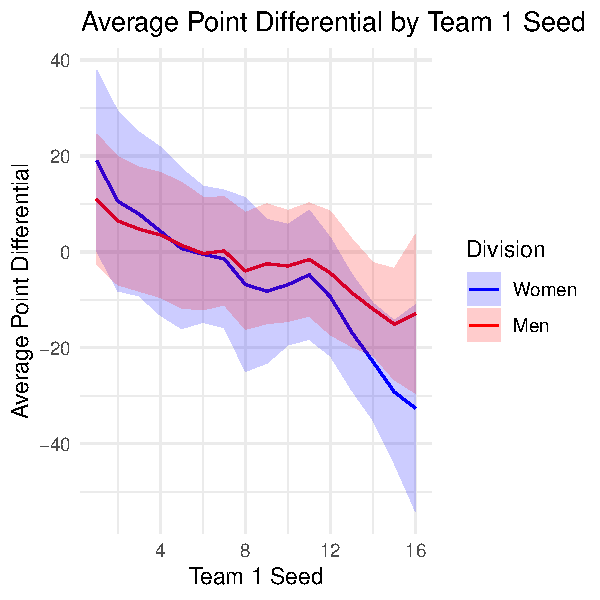
\includegraphics[width=\maxwidth]{figure/unnamed-chunk-1-1} 
\end{knitrout}
\hfill
\begin{knitrout}
\definecolor{shadecolor}{rgb}{0.969, 0.969, 0.969}\color{fgcolor}
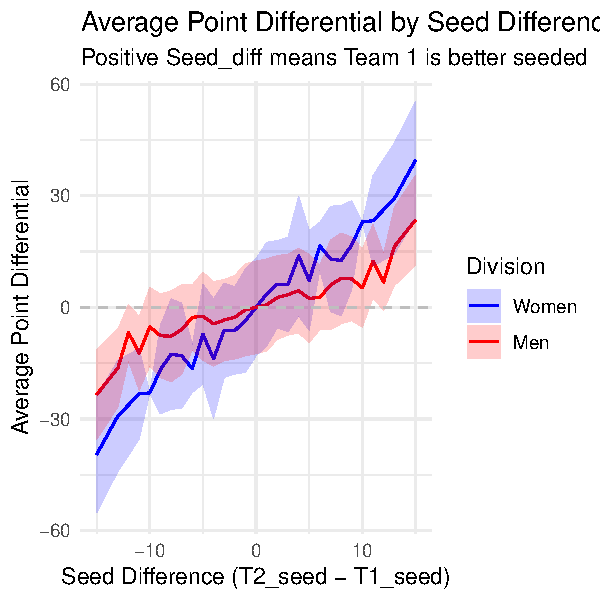
\includegraphics[width=\maxwidth]{figure/unnamed-chunk-2-1} 
\end{knitrout}
\caption{Left: Average point differential by Team 1 seed. Right: Average point differential by seed differential.}
\label{fig:seed_pointdiff}
\end{figure}

The second tier consists of simple season statistics computed from regular season game logs. For each team these include season win percentage, average points scored, average points allowed, and average point differential. Pairwise differentials between Team 1 and Team 2 are also computed for each of these statistics, providing the model with both absolute team quality signals and direct matchup comparison signals. These features capture overall team strength but do not account for the quality of opposition faced. A team that averaged 85 points per game against a weak conference schedule is not necessarily more dangerous than a team that averaged 75 points against a gauntlet of top 25 opponents, and the raw averages alone cannot make that distinction. This limitation motivates the third tier.

The third tier introduces strength of schedule adjusted box score profiles. For each of the fourteen raw box score statistics available in the Kaggle data, including field goals made and attempted, three point attempts, free throw attempts, offensive and defensive rebounds, assists, turnovers, steals, blocks, and personal fouls, seasonal averages are computed from two perspectives. The first perspective captures a team's own offensive and defensive production, prefixed as \texttt{Off\_} and \texttt{Def\_} respectively. The second perspective captures the quality of opposition faced by averaging the seasonal profiles of every opponent a team played during the regular season, producing a set of \texttt{SOS\_} prefixed features. A team whose offensive statistics were produced against consistently strong defensive opponents is credited more heavily than a team whose statistics were inflated by a weak schedule. All box score statistics are adjusted for overtime prior to averaging using the formula $\texttt{adjOT} = \frac{40 + 5 \times \texttt{NumOT}}{40}$, which scales each game's statistics back to a standard 40 minute equivalent. This ensures that high scoring overtime games do not artificially inflate a team's seasonal averages.

The final component of the feature set is a custom Elo rating system developed to capture dynamic team strength across the full regular season. Unlike the static season averages described in the previous tiers, Elo ratings are updated after every game and reflect the cumulative result of a team's performance relative to its opponents throughout the season. This means a team that starts slowly but peaks heading into the tournament will have a higher Elo rating than its season averages alone would suggest, and conversely a team that fades late in the season will have a deflated rating relative to its win percentage.

The Elo system used here is adapted from the rating system originally developed for chess by Arpad Elo \cite{chess}. Each team begins the first season with an initial rating of 1500. After each regular season game the winner gains rating points and the loser loses an equal number, preserving the total rating mass in the system. The magnitude of the exchange depends on how surprising the result was relative to the pre-game expectations implied by the two teams' current ratings. The expected win probability for Team 1 is computed as:

\begin{equation}
E_1 = \frac{1}{1 + 10^{(R_2 - R_1) / 400}}
\end{equation}

where $R_1$ and $R_2$ are the current ratings of Team 1 and Team 2 respectively. The denominator of $400$ is the width parameter that controls how sensitive the expected probability is to rating differences. After the game resolves, ratings are updated as:

\begin{align}
R_1 &= R_1 + k(1 - E_1) \\
R_2 &= R_2 + k(0 - E_2) \\
\end{align}
where $k=64$ is the K-factor controlling the maximum possible rating change per game and $E_2 = 1 - E_1$. When a heavy favorite wins, $E_1$ is close to $1$ and the rating change is small since the result was expected. When a heavy underdog wins, $E_1$ is close to $0$ and the rating change is large. This property makes Elo particularly well suited for tournament prediction because late season upsets and dominant runs cause large rating movements that static averages cannot capture. A key design decision in this implementation is the between-season carry over. Rather than resetting every team to 1500 at the start of each new season, the end of season rating is partially carried forward according to:
\begin{equation}
R_{\texttt{new}} = 0.5 \times R_{\texttt{final}} + 0.5 \times 1500.
\end{equation}

This means 50\$ of a team's historical rating is preserved into the next season while the other 50\% regresses toward the mean. The motivation is that program quality is not purely year to year. A program like Duke or Connecticut that has been consistently elite for two decades should not start each season at the same rating as a mid-major program making its first tournament appearance. The carry over allows the Elo system to accumulate this historical signal while the regression toward the mean prevents ratings from drifting arbitrarily far from the initial value over many seasons.Figures \ref{fig:elo_mens} and \ref{fig:elo_womens} illustrate the end of season Elo ratings for the top 20 men's and women's programs in 2025, reflecting both current season performance and accumulated historical quality. Each team's final end of season Elo rating is included in the feature set as \texttt{T1\_Elo} and \texttt{T2\_Elo}, along with their difference \texttt{Elo\_diff}. Including all three again allows the model to learn both absolute and relative rating effects simultaneously.

\begin{figure}[H]
\centering
\begin{knitrout}
\definecolor{shadecolor}{rgb}{0.969, 0.969, 0.969}\color{fgcolor}
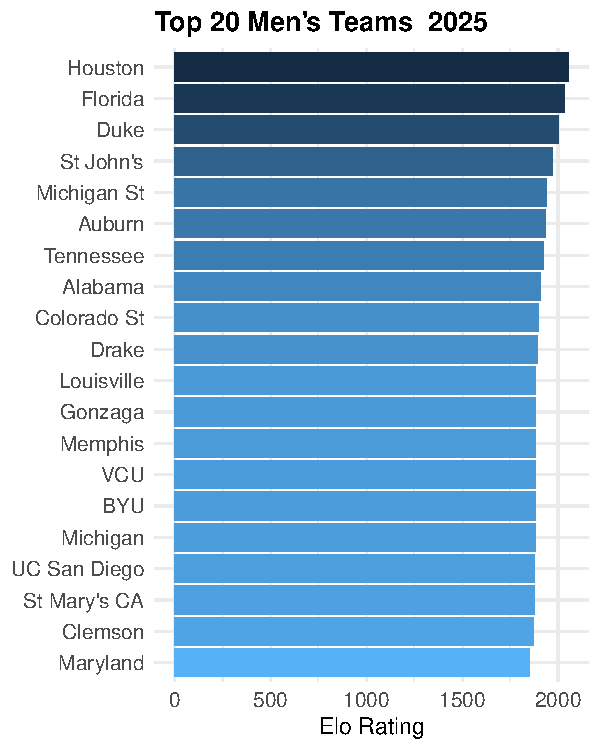
\includegraphics[width=\maxwidth]{figure/unnamed-chunk-3-1} 
\end{knitrout}
\hfill
\begin{knitrout}
\definecolor{shadecolor}{rgb}{0.969, 0.969, 0.969}\color{fgcolor}
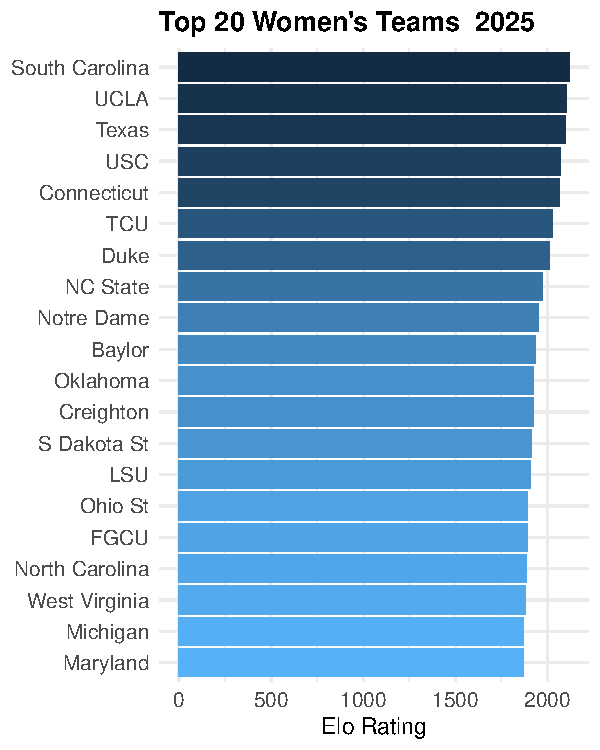
\includegraphics[width=\maxwidth]{figure/unnamed-chunk-4-1} 
\end{knitrout}
\caption{Left: Top 20 men's programs by end of season Elo rating in 2025. Right: Top 20 women's programs by end of season Elo rating in 2025.}
\label{fig:elo_mens}
\end{figure}

%%%%%%%%%%%%%%%%%%%%%%%%%%%%%%%%%%%%%%%%%%%%%%%%%%%%%%%%%%%%%%%%
%%%%%%%%%%%%%%%%%%%%%%%%%%%%%%%%%%%%%%%%%%%%%%%%%%%%%%%%%%%%%%%%
\begin{center}
\section{Point Spread Models}
\end{center}
\thispagestyle{empty} %NO PAGE NUMBER ON SECTION PAGES.
same as above
%%%%%%%%%%%%%%%%%%%%%%
\usubsection{s}
Here are my insights...

\newpage

%%%%%%%%%%%%%%%%%%%%%%%%%%%%%%%%%%%%%%%%%%%%%%%%%%%%%%%%%%%%%%%%
%%%%%%%%%%%%%%%%%%%%%%%%%%%%%%%%%%%%%%%%%%%%%%%%%%%%%%%%%%%%%%%%
\begin{center}
\section{Comparison of models}
\end{center}
\thispagestyle{empty} %NO PAGE NUMBER ON SECTION PAGES.

%%%%%%%%%%%%%%%%%%%%%%

\newpage

%%%%%%%%%%%%%%%%%%%%%%%%%%%%%%%%%%%%%%%%%%%%%%%%%%%%%%%%%%%%%%%%
%%%%%%%%%%%%%%%%%%%%%%%%%%%%%%%%%%%%%%%%%%%%%%%%%%%%%%%%%%%%%%%%
\begin{center}
\section{2026 Competition}
\end{center}
\thispagestyle{empty} %NO PAGE NUMBER ON SECTION PAGES.

%%%%%%%%%%%%%%%%%%%%%%
\usubsection{Strategies}
Here are my insights...
\usubsection{Results}

\newpage

%%%%%%%%%%%%%%%%%%%%%%%%%%%%%%%%%%%%%%%%%%%%%%%%%%%%%%%%%%%%%%%%

\begin{center}
\section{CONCLUSIONS}
\end{center}
\thispagestyle{empty} %NO PAGE NUMBER ON SECTION PAGES.

%%%%%%%%%%%%%%%%%%%%%%
\usubsection{Summary}

As a preliminary assessment...

\clearpage

%%%%%%%%%%%%%%%%%%%%%%%%%%%%%%%%%%%%%%%%%%%%%%%%%%%%%%%%%%%%%%%%


\begin{thebibliography}{99}
\addcontentsline{toc}{section}{REFERENCES} %THIS ADDS REFERENCES TO TABLE OF CONTENTS
\singlespacing %THIS LOOKS BETTER ON REFERENCE PAGE, DOUBLESPACING WOULD BE TOO UGLY
\thispagestyle{empty} %NO PAGE NUMBER ON SECTION PAGES.

\bibitem{Berkowitz2025} S. Berkowitz. NCAA revenue shattered record in 2024, but association faces massive debt from legal settlements. \emph{USA Today}. (2025). Available at https://www.usatoday.com/story/sports/college/2025/02/27/ncaa-financial-report-revenue-surplus/80733616007/

\bibitem{AGA2025} Cohen, Dara. “Americans to Legally Wager Estimated \$3.1 Billion on March Madness - American Gaming Association.” American Gaming Association, 13 Mar. 2025, www.americangaming.org/americans-to-legally-wager-estimated-3-1-billion-on-march-madness/.

\bibitem{Torvik} Torvik, Bart. “T-Rank FAQ.” Blogspot.com, 2017, adamcwisports.blogspot.com/p/every-possession-counts.html.

\bibitem{GD} IBM. “Gradient Descent.” Ibm.com, 7 Oct. 2021, www.ibm.com/think/topics/gradient-descent.

\bibitem{XGBoost} Kavlakoglu, Eda, and Erika Russi. “XGBoost.” Ibm.com, 9 May 2024, www.ibm.com/think/topics/xgboost.

\bibitem{CBS} Boone, Kyle. “How NIL Has Changed College Basketball: Numbers Deep Dive Reveals Surprising Trends, Recipe for Success.” CBSSports.com, 2025, www.cbssports.com/college-basketball/news/how-nil-has-changed-college-basketball-numbers-deep-dive-reveals-surprising-trends-recipe-for-success/.

\bibitem{Optimization} Melis Kizildemir, et al. “A Family of Solutions Related to Shin’s Model for Probability Forecasts.” Journal of Quantitative Analysis in Sports, vol. 21, no. 2, 6 Feb. 2025, pp. 153–158, https://doi.org/10.1515/jqas-2024-0064. Accessed 20 Jan. 2026.

\bibitem{EMH} Burns, William. “Efficient-Market Hypothesis (EMH) | EBSCO.” EBSCO Information Services, Inc. | Www.ebsco.com, 2024, www.ebsco.com/research-starters/social-sciences-and-humanities/efficient-market-hypothesis-emh.

\bibitem{goto} gotoConversion. “GitHub - GotoConversion/Goto\_conversion: Goto\_conversion - Powered $47,000$ of Prize Money, over $10$ Gold Medals and $100$ Medals on Kaggle.” GitHub, 2025, github.com/gotoConversion/goto\_conversion/tree/main. Accessed 20 Jan. 2026.

\bibitem{chess} Glickman, Mark  E., and Thomas Doan. The US Chess Rating System. 26 July 2025, www.glicko.net/ratings/rating.system.pdf.

\bibitem{OLS} Lumivero. “Ordinary Least Squares Regression (OLS).” XLSTAT, Your Data Analysis Solution, 2025, www.xlstat.com/solutions/features/ordinary-least-squares-regression-ols.

\bibitem{logphoto} Kanade, Vijay. “Everything You Need to Know about Logistic Regression.” Spiceworks Inc, Spiceworks, 8 Apr. 2022, www.spiceworks.com/soft-tech/what-is-logistic-regression/.

\bibitem{linearphoto} Raschka, Sebastian. “LinearRegression: An Implementation of Ordinary Least-Squares Linear Regression - Mlxtend.” Rasbt.github.io, rasbt.github.io/mlxtend/user\_guide/regressor/LinearRegression/.

\bibitem{Large Numbers} “Law of Large Numbers | EBSCO.” EBSCO Information Services, Inc. | Www.ebsco.com, 2022, www.ebsco.com/research-starters/mathematics/law-large-numbers.
%IF YOU ARE DOING A PROJECT IN PURE/APPLIED MATH, THEN YOU NEED TO USE AMS STYLE FOR REFERENCES (GET YOUR REFERENCES FROM MATHSCINET). CONSULT YOUR ADVISOR ABOUT WHAT IS THE STANDARD IN YOUR FIELD, IF YOU ARE DOING STATS OR MATH ED.

\bibitem{Pace} “Hoops in Motion: The Evolution of Pace in Basketball.” Substack.com, SLT Sports Analytics: Slamming Data into the Game, Mar. 2024, sltsportsanalytics.substack.com/p/hoops-in-motion-the-evolution-of.

\bibitem{Dean} Oliver, Dean. Basketball on Paper. Potomac Books, 1 Nov. 2004.

\bibitem{logistic} Logistic Regression 12.1 Modeling Conditional Probabilities.

\bibitem{occam} Tavhare, Avadhoot. “Occam’s Razor in Machine Learning: The Principle of Parsimony.” Medium, 21 May 2024, medium.com/@qjbqvwzmg/occams-razor-in-machine-learning-the-principle-of-parsimony-de110ce7fe13.

\bibitem{regularization} “XGBoost Regularization Techniques | XGBoosting.” Xgboosting.com, 2024, xgboosting.com/xgboost-regularization-techniques/.

\end{thebibliography}


 




\end{document} 
